%
% todo: search for citations and add pages when necessary \cite[page]{}
%

%\KOMAoptions{twoside = false} % creates the "dirty hack"-error
\iftoggle{print}{%
  %\KOMAoptions{twoside}
}{
  \KOMAoptions{twoside = false} % creates the "dirty hack"-error
}

%
% \newcommand is used in favor over \set\variable, because the last one overwrittes macros that are already set without a warning
%
\newcommand{\thesisDesignator}{Bachelorarbeit}
\newcommand{\thesisAuthor}{Andreas Linz}
\newcommand{\thesisAuthorEmail}{admin@klingt.net}
\newcommand{\thesisAuthorWebsite}{www.klingt.net}
\newcommand{\thesisAuthorAddress}{Nibelungenring 52\\04279 Leipzig}
\newcommand{\thesisAuthorClass}{10INB-T}
\newcommand{\thesisAuthorCity}{Leipzig}
\newcommand{\thesisUniversity}{HTWK Leipzig}
\newcommand{\thesisUniversityDepartment}{Fakultät für Informatik, Mathematik \& Naturwissenschaften}
\newcommand{\thesisTitle}{Generierung und Design einer Client-Bibliothek für einen RESTful Web Service am Beispiel der Spreadshirt-API}
%\newcommand{\thesisSubtitle}{}
\newcommand{\thesisAdvisor}{Dr. rer. nat. Johannes Waldmann}
\newcommand{\thesisAdvisorSprd}{Jens Hadlich}
\newcommand{\thesisProofreader}{Elisa Jentsch}
\newcommand{\thesisCompany}{Spreadshirt}
\newcommand{\thesisBlankPageText}{Diese Seite wurde mit Absicht leer gelassen.}
\newcommand{\thesisAffidavitName}{Selbständigkeitserklärung}

\pagestyle{empty}

% hack, to "deactivate" link coloring
\hypersetup{
            citecolor=black,
            linkcolor=black,
            urlcolor=black,
            filecolor=black
            }

% PDF meta-data
%\hypersetup{pdfsubject=\subjectname}
%\hypersetup{pdfkeywords=\keywordnames}
\hypersetup{pdftitle=\thesisTitle{}}
\hypersetup{pdfauthor=\thesisAuthor{}}

% Beginn der Titelseite und Verzeichnisse
% roemische Seitennumerrierung
\pagenumbering{Roman}

%\maketitle    
\begin{titlepage}
    %\title{Bachelorthesis}
%\author{Andreas Linz}
%\date{\today}

\begin{center}
    
\includegraphics[width=4cm]{frontpage/HTWK_Logo_schwarz}\\
    \vspace{12pt}
    \large
        \textbf{\thesisUniversity}\\
    \vspace{6pt}
    \normalsize
        \thesisUniversityDepartment\\

    \vspace{24pt}
    \rule{\textwidth}{0.5pt}
    \vspace{12pt}

    \Huge
        Bachelor-Thesis\\
    \vspace{12pt}
    \Large
        \textbf{\thesisTitle}\\
        \ifcsname thesisSubtitle \endcsname
            % exist
            \large
            \thesisSubtitle
        \else
            % don't exist
        \fi
    \vspace{24pt}

    \small
        Author:\\
    \vspace{6pt}
    \large
        \textbf{\thesisAuthor}\\
        \vspace{3pt}
        \normalsize
        \thesisAuthorClass\\
        \href{mailto:\thesisAuthorEmail}{\thesisAuthorEmail}\\
        \thesisAuthorCity, \today\\        

    \vspace{24pt}
    \rule{\textwidth}{0.5pt}
    \vspace{12pt}

    \vfill
    \small
        Gutachter:\\
    \vspace{6pt}
    \large
        \thesisAdvisor\\
    \small
        \thesisUniversity{} -- \thesisUniversityDepartment\\
        \href{mailto:waldmann@imn.htwk-leipzig.de}{waldmann@imn.htwk-leipzig.de}\\
        HTWK Leipzig, F-IMN, Postfach 301166, 04251 Leipzig\\

    \vspace{6pt}
    \large
        \thesisAdvisorSprd\\
    \small
        Spreadshirt HQ, Gießerstraße 27, 04229 Leipzig\\
        \href{mailto:jns@spreadshirt.net}{jns@spreadshirt.net}\\
\end{center}

\end{titlepage}
\blankpage{\thesisBlankPageText}

% zweite Seite mit Angaben zur Arbeit etc. am unteren Ende
\null
\vfill
\begin{flushright}
    \textbf{\thesisAuthor}\\
    \thesisAuthorAddress\\
    \href{mailto:\thesisAuthorEmail}{\thesisAuthorEmail}\\
    \href{http://\thesisAuthorWebsite}{\thesisAuthorWebsite}\\
    \textit{\thesisTitle}\\
    Bachelor Thesis, HTWK-Leipzig, \today
\end{flushright}
\cleardoublepage{}

%
% Selbständigkeitserklärung
%
\setcounter{page}{1}
{    
    \onehalfspacing
    \chapter*{\thesisAffidavitName}

Ich erkläre hiermit, dass ich diese \thesisDesignator{} selbstständig ohne Hilfe Dritter und ohne Benutzung anderer als der angegebenen Quellen und Hilfsmittel verfasst habe. Alle den benutzten Quellen wörtlich oder sinngemäß entnommenen Stellen sind als solche einzeln kenntlich gemacht.\\
Diese Arbeit ist bislang keiner anderen Prüfungsbehörde vorgelegt und auch nicht veröffentlicht worden.\\
Ich bin mir bewusst, dass eine falsche Erklärung rechtliche Folgen haben wird.

{
\vspace{32pt}
\noindent
\hdashrule{5cm}{1pt}{1pt 3pt}\\
\textbf{\thesisAuthor{}}\\
Leipzig, \today
}

}

%
% Danksagungen
%
{    
    \onehalfspacing
    \chapter*{Danksagungen}

%Ein besonderer Dank gilt \thesisAdvisor{} für die Anregungen und Ratschläge sowie das Interesse am Thema.

%Ebenso möchte ich mich bei \thesisAdvisorSprd{} bedanken, der für Fragen jederzeit ein offenes Ohr hatte und mir half den \enquote{roten Faden} bei der Strukturierung der Arbeit nicht zu verlieren. Außerdem gilt \thesisCompany{} ein großer Dank, da sie mir eine wunderbare Arbeitsumgebung sowie nette und hilfreiche Kollegen zur Verfügung gestellt haben.

%Ohne \thesisProofreader{} würde sicherlich der ein oder andere Rechtschreibfehler den Lesefluß trüben, deshalb auch an dieser Stelle , vielen Dank für das Korrekturlesen.
}

%
% Abstract
%
{
    \onehalfspacing
    \chapter*{Abstract}

% todo: Abstract schreiben und schlüsselwörter vervollständigen

% Motivation des Tex
% Fragestellung
% Methodologie
% Ergebnisse
% Implikationen, Schlussfolgerungen

\section*{Schlüsselwörter}

Codegenerierung, RESTful Web Service, Modellierung, Client-Bibliothek, Spreadshirt-API, Polyglot
\newpage
}

\chapter*{Lizenz}

Die vorliegende Bachelorthesis \enquote{\thesisTitle{}} is unter Creative Commons \printhref{http://creativecommons.org/licenses/by-sa/3.0/deed.de}{CC-BY-SA} lizenziert.


% Inhaltsverzeichnis    
%
% manuelles einfuegen eines Lesezeichens im PDF-Index
\cleardoublepage{}
\pdfbookmark[1]{\contentsname}{toc}
\tableofcontents
%\blankpage{\thesisBlankPageText}

%
% Beginn des eigentlichen Inhalts
% arabische Seitennumerrierung
%
% hack to activate link coloring
\hypersetup{
            citecolor=cyan,
            linkcolor=cyan,
            urlcolor=cyan,
            filecolor=cyan
            }

\pagenumbering{arabic}

% headline even on first page of chapter
\renewcommand*{\chapterpagestyle}{chapterStyle}
{           
    % http://www2.informatik.hu-berlin.de/~piefel/LaTeX-PS/Archive-2004/V07-footnote.pdf
    \pagestyle{mainpartStyle}
    \onehalfspacing
    \chapter{Einführung}

\chapterQuote{Essentially, all models are wrong, but some are useful.}{George E. P. Box, Norman R. Draper}{1987}{Empirical Model-Building and Response Surfaces. p. 424}

Die zwei wichtigsten Konstanten in der Anwendungsentwicklung sind laut \parencite{herrington2003code} folgende:
\begin{compactitem}
    \item Die Zeit eines Programmierers ist kostbar
    \item Programmierer mögen keine langweiligen und repetitiven Aufgaben
\end{compactitem}
Codegenerierung greift bei beiden Punkten an und kann zu einer Steigerung der \emph{Produktivität} führen, die mit durch herkömmliches schreiben von Code nicht zu erreichen wäre. 
Änderungen können an zentraler Stelle vorgenommen und durch die Generierung automatisch in den Code übertragen werden, was mit verbesserter \emph{Wartbarkeit} einhergeht.
Die gewonnenen Freiräume kann der Entwickler nutzen um sich mit den Grundlegenden Herausforderungen und Problemen seiner Software zu beschäftigen.
Durch die Festlegung eines Schemas für Variablennamen und Funktionssignaturen, wird eine hohe \emph{Konsistenz}, über die gesamte Codebasis hinweg, erreicht.
Diese Einheitlichkeit vereinfacht auch die Nutzung des Generats\footnote{Ergebnis des Codegenerierungsvorganges}, da beispielsweise nicht mit Überraschungen bei den verwendeten Bezeichnern zu rechnen ist.
Als Eingabe für den Generator dient ein \emph{abstraktes Modell} des betreffenden Geschäftsbereiches. Die Erstellung eines solchen Modells vertieft das Verständnis des Entwicklers für das Geschäftsfeld und gibt gleichzeitig Spezialisten aus dem Fachbereich die Möglichkeit Fragestellungen anhand dieses Modells zu formulieren.
Um die immer kürzeren Entwicklungszyklen einhalten zu können, kann durch Codegenerierung die nötige Effizienzsteigerung geleistet werden.

\section{Spreadshirt}

% Problemstellung
\section{Ziel der Arbeit}

Es ist ein Codegenerator zu erstellen, der aus der abstrakten Beschreibung der \gls{RESTful} Spreadshirt \gls{API} eine Client-Bibliothek erstellt. 

Der Generator soll eine flexible Wahl der Zielsprache bieten, wobei mit \enquote{Zielsprache} im folgenden die Programmiersprache der erzeugten Bibliothek gemeint ist. 
Für das Bibliotheksdesign ist eine \gls{DSL} (Domain-Specific Language) zu realisieren, mit dem Ziel die Nutzung der \gls{API} zu vereinfachen. 

Als Programmiersprache für den Generator wird \emph{Java} verwendet, als Zielsprache der Bibliothek dient \emph{PHP}. Um die gewünschte Flexibilität bezüglich der Zielsprache zu erreichen, wird eine \gls{template-engine} verwendet.

\cref{fig:generatorstructure} stellt den schematischen Aufbau des gewünschten Generators dar.

\begin{tikzpicture}[
    	node distance=12mm and 8mm,
    	every node/.style={font=\scriptsize}
    ]
    % Blocks
    \node(abstract)[greyBlock, double copy shadow]{abstrakte\\API Beschreibung};
    \node(parser)[greyBlock, right=of abstract]{Parser};
    \node(APImodel)[greyBlock, right=of parser]{REST-API\\Modell};
    \node(generator)[greyBlock, right=of APImodel]{Codegenerator\\\textbf{Java}};
    \node(languagemodel)[greyBlock, right= of generator]{Sprachenmodell\\\emph{Abstrakter}\\ \emph{Syntaxbaum}};
    \node(infrastructurecode)[greyBlock, above=of generator]{Infrastrukturcode};
    \node(printer)[greyBlock, right= of languagemodel]{Ausgabemodul};
	\node(bib)[greyBlock, right=of printer]{Client-Bibliothek\\\textbf{php}};
	% Lines  
	\path[arrow, ->] (abstract) -- (parser);
	\path[arrow, ->] (parser) -- (APImodel);
    \path[arrow, ->] (APImodel) -- (generator);
    \path[arrow, ->] (infrastructurecode) -- (generator);
	\path[arrow, ->] (generator) -- (languagemodel);
    \path[arrow, ->] (languagemodel) -- (printer);
    \path[arrow, ->] (printer) -- (bib); 
\end{tikzpicture}

    \chapter{Web Services}
\label{sec:web_services}

\chapterQuote{The purpose of computing is insight, not numbers.}{Richard Hamming}{1962}{Numerical Methods for Scientists and Engineers. Preface}

Dieses Kapitel dient der Begriffserklärung und der Erläuterung weiterer Grundlagen die zum Verständnis dieser Arbeit notwendig sind. Es folgt eine Einführung in die beiden, von der Spreadshirt-API genutzten, Dokumentbeschreibungsformate \gls{XML} und \gls{JSON}. Speziell zu XML werden noch zwei Schemabeschreibungssprachen \gls{XSD} und \gls{RelaxNG} besprochen. Den Schluß bildet die Erläuterung von \gls{REST} und des Webanwendungsbeschreibungsformates \gls{WADL}.

\section{Dokumentbeschreibungsformate}
\label{sec:document_description_formats}

In diesem Abschnitt werden die Dokumentbeschreibungsformate \gls{XML} und \gls{JSON}, der Spreadshirt-API behandelt. Außerdem wird die Schemabeschreibungssprache \emph{XML Schema Description} eingeführt.

\subsection{XML}
\label{sec:xml}

\thesisDefinition{\textsc{Xml}}{
Die \emph{Extensible Markup Language}, kurz \gls{XML}, ist eine Auszeichnungssprache (\enquote{Markup Language}), die eine Menge von Regeln beschreibt um Dokumente in einem mensch- und maschinenlesbaren Format zu kodieren \cite{XML10Specification}.
}

Obwohl das Design von \textsc{Xml} auf Dokumente ausgerichtet ist, wird es häufig für die Darstellung von beliebigen Daten benutzt \cite{wiki:xml}, z.B. um diese für die Übertragung zu serialisieren.

\begin{lstlisting}[
        language=XML, 
        caption=Die gekürzte Antwort der \textsc{API}-Ressource \texttt{users/{userid}/designs/{designID}} als Beispiel für eine \textsc{Xml}-Datei
    ][htb]
<?xml version="1.0" encoding="UTF-8" standalone="yes"?> //@\ding{202}@//
<design xmlns:xlink="http://www.w3.org/1999/xlink" 
        xmlns="http://api.spreadshirt.net" 
        ...>//@\ding{203}@//
    <name>tape_recorder</name>
    ...
    <size unit="px">
        <width>3340.0</width>
        <height>3243.0</height>
    </size>
    <colors/>//@\ding{204}@//
    ...
    <created>
        2013-03-30T12:37:54Z //@\ding{205}@//
    </created>
    <modified>2013-04-02T11:13:02Z</modified>
</design>//@\ding{206}@//
\end{lstlisting}

Eine valide \textsc{Xml}-Datei beginnt mit der \textsc{Xml}-Deklaration \ding{202}. Diese enthält Angaben über die verwendete \textsc{Xml}-Spezifikation und die Kodierung der Datei. 
Im Gegensatz zu gewöhnlichen Tags wird dieses mit \texttt{<?} und mit \texttt{?>} beendet. 
Danach folgen beliebig viele baumartig geschachtelte \emph{Elemente} mit einem Wurzelelement \ding{203}. Die Elemente können Attribute enthalten und werden, wenn sie kein leeres Element sind \ding{204}, von einem schließenden Tag in der gleichen Stufe abgeschlossen \ding{206}. Nicht leere Zeichenketten als Kindelement sind ebenfalls erlaubt \ding{205}.

Mit Hilfe von \emph{Schemabeschreibungssprachen} (siehe \cref{sec:xmlschema}) kann der Inhalt und die Struktur eines Dokumentes festgelegt und gegen diese validiert werden. Der Begriff \textsc{Xml} Schema ist mehrdeutig und wird oft auch für eine konkrete Beschreibungssprache, die \enquote{\textsc{Xml} Schema Definition}, kurz \gls{XSD}, verwendet.


\subsection{JSON}
\label{sec:json}

\thesisDefinition{JSON}{
\emph{Javascript Object Notation}, kurz \emph{JSON}, ist ein leichtgewichtiges, textbasiertes und sprachunbhängiges Datenaustauschformat. Es ist von JavaScript abgeleitet und definiert eine kleine Menge von Formatierungsregeln für die transportable Darstellung (Serialisierung) von strukturierten Daten (nach \cite{JSONRFC}).
}

Im Gegensatz zu XML ist JSON weit weniger mächtig, es gibt z.B. keine Unterstützung für Namensräume und es wird nur eine geringe Menge an Datentypen unterstützt (siehe \cref{tab:jsonDatatypes}). 
Durch seine einfache Struktur wird aber ein deutlich geringerer \enquote{syntaktischer Overhead} erzeugt.
Mit \emph{JSON Schema} \cite{json-schema-draft} ist es möglich eine Dokumentstruktur vorzugeben und gegen diese zu validieren. 

\begin{table}[tb]
    \begin{longtable}[c]{l l}
        \toprule
        \rowcolor{lightgray}
        \textbf{primitiv}   & \textbf{strukturiert}\\
        \midrule
        Zeichenketten       & Objekte\\
        Ganz- und 
        Fließkommazahlen    & Arrays\\
        Booleans            & \\
        null                & \\
        \bottomrule
        \caption{JSON Datentypen}
        \label{tab:jsonDatatypes}
    \end{longtable}
\end{table}

Objekte werden in JSON von geschweiften- \ding{202}, Arrays hingegen von eckigen Klammern begrenzt \ding{203}. 
Objekte enthalten \emph{key-value-pairs} (Schlüssel-Wert-Paare) \ding{204}. Schlüssel sind immer Zeichenketten, die Werte dürfen von allen Typen aus \cref{tab:jsonDatatypes} sein und beliebig tief geschachtelt werden.
%
% wrapping in a minipage prevents the listings block from splitting on pagebreak
%
\begin{lstlisting}[
    language=JavaScript,
    caption=Die gekürzte Antwort der API-Ressource \emph{users/{userid}/designs/{designID}} als Beispiel für eine JSON-Datei
]
{
    "name": "tape_recorder", //@\ding{204}@//
    "description": "",
    "user": { //@\ding{202}@//
        "id": "1956580",
        "href": "http://api.spreadshirt.net/api/v1/users/1956580"
    }, //@\ding{202}@//
    "resources": [ //@\ding{203}@//
    ...
        {
            "mediaType": "png",
            "type": "preview",
            "href": "http://image.spreadshirt.net/image-server/v1/designs/15513946"
        }, 
        ...
    ], //@\ding{203}@//
    "created": "30.03.2013 12:37:54",
    ...
}
\end{lstlisting}    


% ToDo: Titel in Schemasprachen ändern?
\section{XML Schemabeschreibungssprachen (XML Schema)}
\label{sec:xmlschema}

\emph{XML Schema} bezeichnet XML-basierte Sprachen mit denen sich Elemente, Attribute und Aufbau eines XML-Dokumentes beschreiben lassen. 
Ein XML-Dokument wird als \emph{valid/gültig} gegenüber einem Schema bezeichnet, falls die Elemente und Attribute dieses Dokumentes die Bedingungen des Schemas erfüllen \cite{taxonomyXMLSchema}.
Neben XSD (siehe \cref{sec:xsd}) und RelaxNG (siehe \cref{sec:relaxng}) existieren noch weitere Schemasprachen, die hier aber aufgrund ihrer geringen Relevanz nicht behandelt werden. Die beiden hier behandelten Schemasprachen bieten den Vorteil selbst XML-Dokumente zu sein, somit können sie durch herkömmliche XML-Tools bearbeitet werden.

\input{content/basics/web_services/xml_schema/xsd}

\input{content/basics/web_services/xml_schema/relax-ng}


\section{RESTful Web Service}
\label{sec:rest}

\emph{Representational State Transfer} (deutsch: \enquote{Gegenständlicher Zustandstransfer}) ist ein Softwarearchitekturstil für Webanwendungen, welcher von Roy Fielding\footnote{Roy Thomas Fielding, geboren 1965, ist einer der Hauptautoren der HTTP-Spezifikation} in seiner Dissertation aus dem Jahre 2000  beschrieben wurde \cite[Kapitel 5][95 ff.]{fieldingDissertation}. 

Als \gls{RESTful} bezeichnet man dabei eine Webanwendung die den Prinzipien von \gls{REST} entspricht. 

% Diesen Part über die Grundprinzipien verschieben
\subsection{Elemente von REST}

Im folgenden werden die Grundbausteine einer REST-Anwendung erläutert. \Cref{sec:RESTcomponents} beschreibt die Komponenten, die an einer Aktion auf einer \emph{Ressource} beteiligt sind. Dieser Abschnitt basiert auf Kapitel 5.2 von \cite[][S. 86 ff.]{fieldingDissertation}.

\subsubsection{Ressource}

Eine Ressource stellt die wichtigste Abstraktion von Information im REST-Modell dar. Fielding definiert eine \emph{ressource} wie folgt:

\thesisquote{Any information that can be named can be a resource: a document or image, [\ldots]. A resource is a conceptual mapping
to a set of entities, not the entity that corresponds to the mapping at any particular point in
time.}

Eine Ressource kann somit alle Konzepte abbilden die sich über einen Bezeichner referenzieren lassen. Dies können konkrete Dokumente, aber auch Dienste oder sogar Sammlungen von Ressourcen sein.
Außerdem identifiziert ein Ressourcenbezeichner, meist eine \emph{URI} (siehe \cref{sec:unambigiousidentification}), immer dieselbe Ressource, nicht aber deren Wert oder Zustand.

\subsubsection{Repräsentation}

Eine Repräsentation (\emph{representation}) stellt den aktuellen oder den gewünschten Zustand einer Ressource dar. Das Format der Repräsentation ist dabei unabhängig von dem der Ressource, siehe \cref{sec:representationofresources}.
Aktionen mit Komponenten einer REST-API werden durch den Austausch von solchen Repräsentationen durchgeführt.

Im Allgemeinen wird unter einer Repräsentation nur eine Folge von Bytes verstanden, inklusive \emph{Metainformationen} welche den Inhalt der Bytefolge klassifiziert, sowie \emph{Kontrolldaten} die die gewünschte Aktion oder die Bedeutung der Anfrage beschreiben. Letztere sind meist HTTP-Header-Felder\footnote{für die HTTP-Header-Definitionen siehe \url{http://www.w3.org/Protocols/rfc2616/rfc2616-sec14.html\#sec14.43}}, bspw. um das Cachingverhalten zu ändern.

\begin{minipage}{\textwidth}
    \begin{lstlisting}[
        language=XML,
        caption=Beispiel zu Metainformationen für REST-Repräsentation aus WADL-Datei der Spreadshirt-API,
        label=lst:metainformationREST
        ]
    ...
    <response>
        <representation xmlns:sns="http://api.spreadshirt.net",
            element="sns:productTypes" status="200", //@{\ding{202}}@//
            mediaType="application/xml"> //@{\ding{203}@//
            <doc title="Success"/>
        </representation>
        ...
    </response>
    \end{lstlisting}
\end{minipage}

Ein Beispiel für eine solche Angabe von Metainformationen ist in \Cref{lst:metainformationREST} zu finden, \ding{202} zeigt dies in Form einer \emph{Typangabe} und \ding{203} eines \emph{mediaType}-Attributes.

\subsubsection{Konnektoren}

Konnektoren stellen eine Schnittstelle für die Kommunikation mit Komponenten der REST-Webanwendung dar. Aktionen auf Ressourcen und der Austausch von Repräsentationen finden über diese Schnittstellen statt. Der Konnektor bildet die Parameter der Schnittstelle auf das gewünschte Protokoll ab.

Eingangsparameter\footnote{\textperiodcentered optionaler Parameter}:
\begin{compactitem}
    \item Anfrage-Kontrolldaten
    \item Ressourcenidentifizierung (Ressourcenbezeichner)
    \item[\textperiodcentered] Repräsentation der Ressource
\end{compactitem}
Ausgangsparameter:
\begin{compactitem}
    \item Antwort-Kontrolldaten
    \item[\textperiodcentered] Metainformationen
    \item[\textperiodcentered] Repräsentation der Ressource
\end{compactitem}

\Cref{tab:RESTconnectors} listet Beispiele für Konnektoren auf.

\begin{table}[tb]
    \begin{longtable}[c]{l l}
        \toprule
        \rowcolor{lightgray}
        \textbf{Konnektor}   & \textbf{Beispiel}\\
        \midrule
        client      & libwww\\
        server      & libwww, Apache HTTP-Server API\\
        cache       & browser cache, Akamai\\
        resolver    & bind\\
        tunnel      & SOCKS\\
        \bottomrule
        \caption{Beispiele für Konnektoren nach \cite{fieldingDissertation}}
        \label{tab:RESTconnectors}
    \end{longtable}
\end{table}       

\subsubsection{Komponenten}
\label{sec:RESTcomponents}

\begin{description}
    \item[Ursprungsserver] 
        Serverseitiger Konnektor der den Namespace der angeforderten Ressource verwaltet. Er ist die einzige Quelle für Repräsentationen, sowie der endgültige Empfänger von Änderungsanfragen an seine Ressourcen. (siehe \cref{sec:unambigiousidentification}).
    \item[Proxy] Zwischenkomponente die explizit vom Client verwendet kann, aus Sicherheits-, Performance- oder Kompatibilitätsgründen.
    \item[Gateway] Dient als Schnittstelle zwischen Client- und Servernetzwerk, kann zusätzlich aus den gleichen Gründen wie der Proxy verwendet werden. Konträr zum Proxy kann der Client aber nicht entscheiden ob er einen Gateway nutzen möchte.
    \item[User Client] 
        Ein clientseitiger \emph{Konnektor}, der die Anfrage an die API startet und einziger Empfänger der Antwort ist. In den meisten Fällen ist dies einfach ein \emph{Webbrowser}.
\end{description}

\subsection{REST-Prinzipien}

Die fünf Grundlegenden REST-Prinzipien, nach \cite[11 ff.]{Tilkov09}:
\begin{compactitem}
    \item Ressourcen mit eindeutiger Indentifikation
    \item Verknüpfungen / Hypermedia
    \item Standartmethoden (siehe \cref{sec:standardmethods})
    \item unterschiedliche Repräsentationen
    \item statuslose Kommunikation
\end{compactitem}

\subsubsection{Eindeutige Identifikation}
\label{sec:unambigiousidentification}

Um eine \emph{eindeutige Identifikation} zu erreichen, wird jeder Ressource eine \gls{URI} vergeben. Dadurch ist es möglich zu jeder verfügbaren Ressource einen Link zu setzen. 
Nachfolgend eine Beispiel-URI, um den Artikel 42 aus dem Warenkorb 84 anzusprechen:
\[
    \underbrace{http://api.spreadshirt.net/api/v1/}_{Basis-URL}\underbrace{\overbrace{baskets/84}^{Warenkorb}\overbrace{/item/42}^{Artikel}}_{Ressource}
    \label{RESTexampleURL}
\]

\subsubsection{Hypermedia}
\label{sec:hypermedia}

Innerhalb einer Ressource kann auf weitere verlinkt werden (\emph{Hypermedia}). Als Nebeneffekt der eindeutigen Identifikation durch \glspl{URI} sind diese auch außerhalb des Kontextes der aktuellen Anwendung gültig. 

Das Folgen eines Links entspricht dabei einer Zustandsänderung innerhalb der Anwendung.
Die vorhandenen Verknüpfungen legen fest welche Zustandsübergänge  erlaubt sind.

\subsubsection{Standardmethoden}
\label{sec:standardmethods}

Durch die Nutzung von \emph{Standardmethoden} ist abgesichert das eine Anwendung mit den Ressourcen arbeiten kann, vorausgesetzt sie unterstützt diese. 

\gls{REST} ist nicht auf HTTP beschränkt, praktisch alle REST-APIs nutzen aber dieses Protokoll. HTTP umfasst dabei folgende Methoden\footnote{Kapitel 9 des HTTP 1.1 RFC2616 beschreibt diese inklusive \emph{TRACE} und \emph{CONNECT} umfassend \cite{HTTP11RFC}}:
\begin{compactitem}
    \item GET
    \item PUT
    \item POST
    \item DELETE
    \item HEAD
    \item OPTIONS
\end{compactitem}

Alle bis auf \emph{POST} und \emph{OPTIONS} sind \emph{idempotent} (\cite{HTTP11RFC} Kapitel 9), d.h. eine hintereinander Ausführung der Methode führt zu demselben Ergebnis wie ein einzelner Aufruf. Dies bedeutet das sich ein \emph{RESTful Web Service} serverseitig ebenso verhalten muss.

\subsubsection{Repräsentationen von Ressourcen}
\label{sec:representationofresources}

Die Repräsentation sollte unabhängig von der Ressource sein, um die Darstellung gegebenenfalls für den Client anzupassen. 
Die Client-Anwendung kann dadurch mittels \emph{Query-Parameter} oder als Information im \emph{HTTP-Header} das gewünschte Format angeben und erhält die entsprechend formatierte Antwort.
Anhand des \emph{Content-Type} Feldes aus dem HTTP-Header kann der Client das Format der Antwort überprüfen, für \gls{JSON} lautet dies bspw. \texttt{application/json}.

\subsubsection{Statuslose Kommunikation}
\label{sec:stateless_communication}

Es soll kein Sitzungsstatus (\emph{session-state}) vom Server gespeichert werden, d.h. jede Anfrage des Client muss alle Informationen enthalten, die nötig sind um diese serverseitig verarbeiten zu können. Der Sitzungstatus wird dabei vollständig vom Client gehalten. 
Diese Restriktion führt zu einigen Vorteilen:
\begin{compactitem}
    \item Verringerung der Kopplung zwischen Client und Server
    \item zwei aufeinanderfolgende Anfragen können von unterschiedlichen Serverinstanzen beantwortet werden
    \item[$\hookrightarrow$] verbesserte Skalierbarkeit
\end{compactitem}

Daraus resultiert eine erhöhte Netzwerklast, da die Statusinformationen bei jeder Anfrage mitgesendet werden müssen.


\section{WADL}
\label{sec:wadl}

Die \emph{Web Application Description Language} (kurz \gls{WADL}) ist eine maschinenlesbare Beschreibung einer \gls{HTTP}-basierten Webanwendung einschließlich einer Menge von \gls{XML} Schematas \cite{hadleyWADL}.
Die aktuelle Revision ist vom \citedate{WADLcurrent} \cite{WADLcurrent}. Im weiteren beziehe ich mich aber auf die in der Spreadshirt-\gls{API} verwendeten Version, datiert am 9. November 2006. Die Unterschiede zwischen beiden Revisionen können unter \cite{WADLchanges} nachvollzogen werden.

Die Beschreibung eines Webservices durch \gls{WADL} besteht nach \cite{hadleyWADL} im groben aus den folgenden vier Bestandteilen (eigene Übersetzung):
\begin{description}
     \item[Menge von Ressourcen] Analog einer Sitemap, also die Übersicht aller verfügbaren Ressourcen
     \item[Beziehungen zwischen Ressourcen] die kausale und referentielle Verknüpfung zwischen Ressourcen
     \item[Methoden die auf Ressourcen angewendet werden können] die von der jeweiligen Ressource unterstützten [\gls{HTTP}]-Methoden, deren Ein- und Ausgabe, sowie die unterstützten Formate
     \item[Ressourcenrepräsentationen] die unterstützten \gls{MIME}-Typen und verwendeten Datenschemata (\cref{sec:xsd})
\end{description} 

\newpage

\begin{minipage}{\textwidth}
\begin{lstlisting}[language=XML, caption={Beispielaufbau einer \gls{WADL}-Datei anhand der Spreadshirt-\gls{API} Beschreibung}, label=lst:wadlstructure, name=wadlstructure]
<?xml version="1.0" encoding="UTF-8" standalone="yes"?> //@\ding{202}@//
<application xmlns="http://research.sun.com/wadl/2006/10"> //@\ding{203}@//
    <grammars> //@\ding{204}@//
        <include href="http://api.spreadshirt.net/api/v1/metaData/api.xsd">
            <doc>Catalog XML Schema.</doc>
        </include>
        ...
    </grammars>
    <resources base="http://api.spreadshirt.net/api/v1/"> //@\ding{205}@//
        <resource path="users/{userId}"> //@\ding{206}@//
            <doc>Return user data.</doc>
            <method name="GET"> //@\ding{207}@//
                <doc>...</doc>
                <request> //@\ding{208}@//
                    <param 
                        xmlns:xsd="http://www.w3.org/2001/XMLSchema" 
                        name="mediaType" 
                        style="query" 
                        type="xsd:string">
                    <doc>...</doc>
                    </param>
                    ...
                </request>
                <response> //@\ding{209}@//
                    <representation 
                        xmlns:sns="http://api.spreadshirt.net"
                        element="sns:user" 
                        status="200" 
                        mediaType="application/xml">
                    <doc title="Success"/>
                    </representation>
                    <fault status="500" mediaType="text/plain">
                        <doc title="Internal Server Error"/>
                    </fault>
                    ...
                    }
                ...
</application>
\end{lstlisting}
\end{minipage}

Die Datei beginnt mit der Angabe der \gls{XML}-Deklaration \ding{202}.
Die Attribute des Wurzelknotens \texttt{<application>} enthalten \emph{namespace} Definitionen, u. a. auch den der verwendeten \gls{WADL}-Spezifikation \ding{203}.
Innerhalb des \texttt{<grammars>} Elements werden die benutzten \gls{XML} Schemas angegeben \ding{204}. 
Um die Ressourcen der Webanwendung ansprechen zu können, wird noch die Angabe der Basisadresse benötigt \ding{205}. 
Innerhalb des \texttt{<resources>} Elements findet sich die Beschreibung der einzelnen Ressourcen. Diese sind gekennzeichnet durch eine zur Basisadresse relativen \gls{URI} \ding{206}. In \texttt{\{\ldots\}} eingeschlossene Teile einer \gls{URI} werden durch den Wert des gleichnamigen \emph{request} Parameters ersetzt um die \gls{URI} zu bilden (generative \glspl{URI}).
Im Folgenden werden die von der Ressource unterstützten \gls{HTTP}-Methoden beschrieben \ding{207}, deren Anfrageparameter \texttt{<request>} \ding{208} sowie die möglichen Ausgaben der jeweiligen Methode \texttt{<response>} \ding{209}.

Die Dokumentations-Tags \texttt{<doc>} sind für alle \gls{XML}-Elemente optional.
Um das Listing nicht unnötig zu verlängern, wurden die schließenden \emph{Tags} weggelassen.

\Cref{fig:wadlstructure} zeigt die baumartige Struktur einer \gls{WADL}-Datei. Die Kanten enthalten Informationen über Kardinalität oder die Form des Elements (Definition/Referenz). Innerhalb der Elemente sind deren Attribute aufgelistet, oder \enquote{\ldots} falls diese schon aufgelistet wurden.

\newpage

\begin{figure}
    \centering
    \resizebox{!}{1.1\textwidth}{
        \begin{tikzpicture}[
    level 1/.style={
        font=\large,
        sibling distance=4cm,
        level distance=5cm
    },
    level 2/.style={
        font=\normalsize,
        level distance=4.5cm,
        sibling distance=7cm
    },
    level 3/.style={
        font=\small,
        level distance=4cm,
        sibling distance=2cm
    },
    level 4/.style={
        level distance=3cm,
        sibling distance=2cm
    }
    edge from parent/.style={
        draw=black,
        shorten >=5mm,
        shorten <=5mm
    },
    edgeText/.style={
        sloped,
        near end,
        above
    },    
    centeredEdgeText/.style={
        sloped,
        above
    },                
    every two node part/.style={
        color=magenta,
        font=\scriptsize,
        align=left
    },
    element/.style={
        rectangle,
        rounded corners,
        draw=gray,
        very thick
    },
    splitElement/.style={
        rectangle,
        rounded corners,
        draw=gray,
        very thick,
        rectangle split, 
        rectangle split parts=2
    }
]
\node {\Large \textbf{application}}
child {
    node [splitElement] {
        doc
        \nodepart{two}
        xml:lang\\
        title
    }
    edge from parent node[edgeText] {0..*};
}
child {
    node [element] {grammars}
    child [level distance = 2.5cm] {
        node [splitElement] {
            include
            \nodepart{two}
            href
        }
        edge from parent node[edgeText] {0..*};
    }
    edge from parent node[edgeText] {0..1};
}
child {
    node [splitElement] {
        resources
        \nodepart{two}
        base
        }
    child [sibling distance=6cm] {
        node [splitElement] {
            resource\_type
            \nodepart{two}
            id
        }
        child {
            node [splitElement] {
                doc
                \nodepart{two}
                \ldots
            }
            edge from parent node [edgeText] {0..*};
        }
        child {
            node [splitElement] {
                param
                \nodepart{two}
                id\\
                name\\
                style\\
                type\\
                default\\
                path\\
                required\\
                repeating\\
                fixed
            }
            child {
                node [splitElement] {
                    option
                    \nodepart{two}
                    value
                }
                child {
                    node [splitElement] {
                        doc
                        \nodepart{two}
                        \ldots
                    }
                    edge from parent node [edgeText] {0..*};
                }
            }
            child {
                node [splitElement] {
                    link
                    \nodepart{two}
                    resource\_type\\
                    rel\\
                    rev\\
                    location\\
                    index
                } 
                edge from parent node [edgeText] {0..*};
            }
            edge from parent node [edgeText] {0..*};
        }
        child {
            node [splitElement] {
                method
                \nodepart{two}
                \ldots
            }
            edge from parent node [edgeText] {0..*};
        }
        edge from parent node [edgeText] {0..*};
    }
    child {
        node [splitElement] {
            resource
            \nodepart{two}
            id\\
            path\\
            type\\
            queryType
            }
        child {
            node [splitElement] {
                doc
                \nodepart{two}
                \ldots
            }
            edge from parent node[edgeText] {0..*};       
        }
        child  {
            node [splitElement] {
                param
                \nodepart{two}
                \ldots
                }
            edge from parent node[edgeText] {0..*};                    
        }
        child {
            node [splitElement] {
                method
                \nodepart{two}
                \ldots
            }
            edge from parent node[edgeText] {0..*};                    
        }
        child {
            node [splitElement] {
                resource
                \nodepart{two}
                \ldots
            }
            edge from parent node[edgeText] {0..*};
        }
        edge from parent node [edgeText] {0..*};                                
    }
    edge from parent node[edgeText] {0..1};
}
child {
    node [element] {resource\_type}
    edge from parent node [edgeText] {0..*};
}            
child [level distance = 6cm] {
    node [element] {method}
    child [sibling distance = 3cm] {
        node [splitElement] {
            method
            \nodepart{two}
            href
        }
        edge from parent node [centeredEdgeText] {reference};
    }
    child [sibling distance = 3cm, level distance=6cm] {
        node [splitElement] {
            method
            \nodepart{two}
            name\\
            id
        }
        child [sibling distance = 2.5cm] {
            node [element] {request}
            child {
                node [element, rectangle split, rectangle split parts=2, align=left] {
                    representation
                    \nodepart{two}
                    \color{green!50!black}
                    nur PUT \& POST\\
                    \ldots
                }
                edge from parent node [edgeText] {0..*};                 
            }
            child {
                node [splitElement] {
                    doc
                    \nodepart{two}
                    \ldots
                }
                edge from parent node [edgeText] {0..*};
            }
            child {
                node [splitElement] {
                    param
                    \nodepart{two}
                    \ldots
                }
                edge from parent node [edgeText] {0..*};
            }
            edge from parent node [edgeText] {0..*};
        }
        child {
            node [splitElement] {
                doc
                \nodepart{two}
                \ldots
            }
            edge from parent node [edgeText] {0..*};
        }
        child [sibling distance = 2.5cm, level distance = 7cm] {
            node [element] {response}
            child {
                node [splitElement] {
                    doc
                    \nodepart{two}
                    \ldots
                }
                edge from parent node [edgeText] {0..*};
            }
            child {
                node [splitElement] {
                    representation
                    \nodepart{two}
                    \ldots
                }
                edge from parent node [edgeText] {0..*};
            }
            child {
                node [splitElement] {
                    fault
                    \nodepart{two}
                    \ldots
                }
                edge from parent node [edgeText] {0..*};
            }
            child {
                node [splitElement] {
                    param
                    \nodepart{two}
                    \color{green!50!black}                    
                    style=header
                    \\
                    \ldots
                }
                edge from parent node [edgeText] {0..*};
            }
            edge from parent node [edgeText] {0..*};
        }
        edge from parent node [centeredEdgeText] {declaration};
    }
    edge from parent node [edgeText] {0..*};
}           
child {
    node [element] {representation}
    child [sibling distance = 3cm,level distance=2.5cm] {
        node [splitElement] {
            representation
            \nodepart{two}
            href
        }
        edge from parent node [centeredEdgeText] {reference};
    }
    child [sibling distance = 3cm, level distance=3.5cm] {
        node [splitElement] {
            representation
            \nodepart{two}
            id\\
            mediaType\\
            element\\
            profile []\\
            status []
        }
        child {
            node [splitElement] {
                param
                \nodepart{two}
                \ldots
            }
            edge from parent node [edgeText] {0..*};
        }
        edge from parent node [centeredEdgeText] {definition};
    }
    edge from parent node [edgeText] {0..*};
}           
child {
    node [splitElement] {
        fault
        \nodepart{two}
        \color{green!50!black}
        entspricht \emph{representation}
    }
    edge from parent node [edgeText] {0..*};
}
;
\end{tikzpicture}  
    }
    \caption{Struktur einer \gls{WADL}-Datei, nach Kapitel 2 \cite{hadleyWADL}}
    \label{fig:wadlstructure}
\end{figure}


    \chapter{Codegenerierung}
\label{chap:codegeneration}

\chapterQuote{All problems in computer science can be solved by another level of indirection.}{\citeauthor{Wilson}}{\citeyear{Wilson}}{\cite[][Kapitel 17]{Wilson}}

% Todo: Kapiteleinleitung für Generatoren und Modellierung
Im folgenden Kapitel werden grundlegende Begriffe im Zusammenhang mit Codegeneratoren und Datenmodellen definiert, zusätzlich wird eine Übersicht über gebräuchliche Generatorformen, dessen Aufgaben und Arten der Optimierung durch den Generator, gegeben. 
\Cref{sec:datamodel} \ldots

%Generative Programming p. 333
%todo: \cite{czarnecki2000generative} in der Kapiteleinleitung erwähnen um sich wiederholende Referenzen zu vermeiden

\begin{thesisDefinition}[Codegenerator]
Ein \emph{Codegenerator} ist ein Programm, welches aus einer höhersprachigen Spezifikation\footnote{m. a. W.: auf einem höheren Abstraktionslevel als die zur Implementierung verwendete Programmiersprache} einer Software oder eines Teilaspektes, die Implementierung erzeugt (nach \cite{czarnecki2000generative}).
\end{thesisDefinition}

% todo: folgende Liste entfernen?
Generatoren widmen sich drei wichtigen Problemen\cite{czarnecki2000generative}:
\begin{description}[style=nextline]
    \item[Relevanz von Systembeschreibungen erhöhen] Eine Systembeschreibung sollte direkt und explizit die Anforderungen bestimmen und mit der Sprache der Problemdomäne formuliert sein.
    \item[Erzeugung einer effizienten Implementierung] Die größte Herausforderung bei der Erstellung eines Generators liegt in der Abbildung von der Spezifikation zur Implementierung, da es meist keine direkte Übereinstimmung zwischen beiden Konzepten gibt.
    \item[\enquote{Library scaling problem}] Nur die durch die Spezifikation benötigten Methoden generieren.
\end{description}

% todo: Satz ändern, quasi nur Übersetzung, Code-Transformatoren nicht erklärt
Der Begriff \enquote{Generator} ist sehr allgemein und wird für verschiedene Technologien verwendet, wie \emph{Compiler}, \emph{Präprozessoren}, \emph{Metafunktionen} (Template-Metaprogramming in C++), \emph{Codetransformatoren} und natürlich \emph{Codegeneratoren}.

\section{Aufgaben eines Generators}
\begin{compactenum}
    \item Validieren der Spezifikation
    \item Spezifikation durch Vorgabewerte vervollständigen
    \item Optimierungen vornehmen
    \item Implementierung erzeugen
\end{compactenum}

Je nach Form der Spezifikation, muss diese durch einen Analyse-Schritt (\emph{parsing}) in die interne Darstellung des Generators überfürht werden, bspw. bei einem Compiler in einen \emph{Abstrakten Syntaxbaum} (siehe \cref{sec:ast}).
Der Informationsgehalt der Spezifikation ist ausschlaggebend für den Grad der zu erreichenden Automatisierung.

\section{Vorteile für den Entwickler}

Die folgende Auflistung basiert ebenfalls auf \cite[][S. 15]{czarnecki2000generative}.

\begin{description}
    \item[Qualität]
        Bugfixes und Verbesserungen werden durch das Generatorsystem in die gesamte Codebasis propagiert.
    \item[Konsistenz]
        Durch ein vorgegebenes Schema für die Schnittstellen- und Variablenbezeichner wird eine hohe Einheitlichkeit erreicht.
    \item[zentrale Wissensbasis]
        % todo: Metamodell erklären
        Das domänenspezifische Wissen wird in dem Metamodell gebündelt, das dem Generator als Eingabe dient. Änderungen am Modell werden durch den Generator in die gesamte Codebasis eingepflegt.
    \item[signifikantere Designentscheidungen]
        Aufgrund des verringerten Implementierungsaufwandes kann der Entwickler mehr Zeit für das Design seiner Architektur , API etc. verwenden. Designfehlentscheidungen können durch Änderungen an den Templates korrigiert werden und bedürfen somit keiner manuellen Korrektur aller generierten Klassen.
\end{description}

Die Erstellung eines Generatorsystems geht mit einem nicht unerheblichen Aufwand einher, dieser sollte in Relation zum Umfang des zu erzeugenden Codes gesehen werden.
Ist der Umfang des Erzeugnisses zu gering, kann der Aufwand zur Entwicklung einer Generatorlösung kontraproduktiv sein.

\section{Generatorformen}

Eine Form der Klassifikation von Codegeneratoren ist nach der Menge des erzeugten Codes:

\begin{table}[htb]
    \begin{longtable}[c]{l l l}
        \toprule
        \rowcolor{lightgray}
        \textbf{teilweise}   & \textbf{vollständig}     & \textbf{mehrfach}\\
        \midrule
        Inline-Code Expander    & Tier-Generator    & n-Tier Generator\\
        Mixed-Code Generator & &\\
        Partial-Class Generator & & \\
        \bottomrule
        \caption{Generatoren Klassifikation nach Generierungsmenge}
        \label{tab:generatorclassification}
    \end{longtable} 
\end{table}

Generatorformen nach \cite{herrington2003code}:
\begin{description}
    \item[Inline-Code Expander]
        Ein Inline-Code Expander nimmt Quellcode als Eingabe und ersetzt spezielle Mark-Up Sequenzen durch seine Ausgabe. Die Änderungen werden hierbei nicht in das Quellfile übernommen sondern meist direkt zu dem Compiler oder Interpreter weitergeleitet.
    \item[Mixed-Code Generator]
        Der Mixed-Code Generator arbeitet grundsätzlich wie der Inline-Code Expander, seine Änderungen werden aber in die Quelle zurückgeschrieben.
    \item[Partial-Class Generator]
        Partial-Class Generatoren erzeugen aus einer abstrakten Beschreibung und Templates einen Satz von Klassen, diese bilden aber nicht das vollständige Programm sondern werden durch manuell erzeugten Code vervollständigt. % todo: manuell erzeugt = handgeschrieben?
    \item[Tier-Generator]
        Die Arbeitsweise des Stufen- oder Tier\footnote{Tier, zu deutsch \enquote{Stufe}}-Generators entspricht der des Partial-Class Generators, mit der Ausnahme das vollständiger Code erzeugt wird, der keiner Nacharbeit bedarf.\footnote{Der im Laufe dieser Arbeit entwickelte Generator entspricht diesem Schema.}
    \item[$n$-Tier Generator] 
        Ein $n$-Tier Generator erzeugt neben dem eigentlichen Quellcode noch beliebige andere Informationen, bspw. eine Dokumentation oder Testfälle.
\end{description}

Die Entwicklung einer \enquote{Full-Domain Language} stellt die oberste Stufe der Generatorformen dar. Eine solche Sprache ist Turing-vollständig und speziell auf die Problemdomäne ausgerichtet.

\section{Optimierung durch den Generator}

Die Effektivität von Optimierungen steigt mit dem Abstraktionslevel, deshalb ist es ratsam diese vom Generator durchführen zu lassen. Im Gegensatz zum Compiler, der viele dieser Optimierungen auch selbst durchführt, besitzt der Generator domänenspezifisches \enquote{Wissen} (\emph{domain-specific optimization}) und kann teilweise ohne Abhängigkeiten der Zielsprache optimieren.

Nachfolgend eine Auflistung möglicher Optimierungen:
% global optimizations?

\begin{description}[style=nextline]
\item[Inlining]
    Ein Symbol durch seine Definition ersetzen oder anstelle eines Funktionsaufrufes, die Deklaration der Funktion selbst einfügen.
\item[Constant folding]
    Auswertung von Ausdrücken deren Operanden während der \emph{compile time} bekannt sind.
\item[Data caching]
    Anstatt mehrfach denselben Ausdruck auszuwerten, das Ergebnis einmal berechnen und darauf an anderer Stelle referenzieren.
\item[Loop fusion]
    Zusammenführen von Schleifen, die über den gleichen Bereich iterieren und deren Schleifenkörper unabhängig voneinander ist.
\item[Loop unrolling]
    Die Schleife durch $n$-mal deren Inhalt ersetzen, wobei $n$ die Anzahl der Iterationen ist.
\item[Code motion]
    Invariante\footnote{unveränderliche} Codebereiche aus dem Schleifenkörper herausnehmen.
\item[Dead-code elimination]
    Entfernen von ungenutzten Variablen und unerreichbaren Codebereichen.
\item[Partial evaluation/Specialisation]
    \emph{Partial evaluation} oder auch \emph{Specialisation} meinen das Erzeugen von spezialisierten Funktionen. Diese implementieren statische Eingaben mit dem Ziel einer kleineren Funktionssignatur.
\item[Parallelization]
    Analyse der Datenabhängigkeit durch den Generator und eventuelles parallelisieren voneinander unabhängiger Bereiche.
\end{description}


\section{Datenmodell}
\label{sec:datamodel}

% todo: Spezifikation oder domänenspezifisches Modell?
Das Datenmodell enthält die Informationen der Spezifikation und dient als Eingabe für den Generator, es ist somit die \emph{Basis der Codegenerierung}. \citeauthor{rfc3198} definieren den Begriff in \cite{rfc3198} folgenderweise\footnote{eigene Übersetzung}:

\thesisDefinition{Datenmodell}{
    Ein Datenmodell ist im Grunde die Darstellung eines Informationsmodells unter Berücksichtigung einer Menge von Mechanismen für die Darstellung, Organisierung, Speicherung und Bearbeitung von Daten.
    Das Modell besteht aus einer Sammlung von \ldots
    \begin{compactitem}
        \item{Datenstrukturen, wie Listen, Tabellen, Relationen etc.}
        \item{Operationen die auf die Strukturen angewendet werden können, wie Abfrage, Aktualisierung, ...}
        \item{Integritätsbedingungen die gültige Zustände (Menge von Werten) odder Zustandsänderungen (Operationen auf Werten) definieren.}
    \end{compactitem}
}

Bei dieser Definition wird der Begriff \emph{Informationsmodell} genutzt, er beschreibt die Informationen die im Datenmodell abgebildet werden sollen ohne Berücksichtigung softwaretechnischer Aspekte. Das Informationsmodell stellt somit die \enquote{natürlichen Daten} dar.

Bei einem Codegenerator entspricht das Datenmodell der internen Darstellung der Spezifikation. Neben den direkt in der Spezifikation enthaltenen Informationen kann der Generator im Analyseschritt (siehe \cref{sec:generator_tasks}) bspw. Datenabhängigkeiten erkennen und diese zur Optimierung nutzen oder das interne Datenmodell damit anreichern. Das \emph{erkennen von Semantik} im Eingabemodell ist aber nicht auf Datenabhängigkeiten beschränkt sondern kann auf beliebige Beziehungen ausgeweitet werden. 

Wie man in \Cref{fig:wadlstructure} erkennen kann, entspricht die Struktur einer WADL-Datei einem Baum. Aus diesem Grund eignet sich eine Baumstruktur für das Datenmodell des Generators besonders gut. Um die Zielsprache (siehe \cref{sec:target_language}) im internen Datenmodell abbilden zu können, wird ein \gls{AST} als Datenstruktur gewählt.

\subsection{Abstract Syntax Tree (AST)}
\label{sec:ast}

Eine anschauliche Definition bietet \cite[][S. 69]{ahoCompiler} (eigene Übersetzung):
\thesisDefinition{Abstract Syntax Tree -- \citeauthor{ahoCompiler}}{
Ein Abstrakter Syntaxbaum ist die Darstellung eines Ausdrucks, wo jeder Knoten einen \emph{Operator} und dessen Kindknoten die \emph{Operanden} repräsentieren.
Im Allgemeinen kann für jedes Programmierkonstrukt ein Operator erzeugt werden, dessen semantisch bedeutsamen Komponenten dann als Operanden gehandhabt werden.
}

%Etwas kürzer definiert \citeauthor{gruneCompiler} den Begriff in \cite[][S. 9 ff.]{gruneCompiler} (eigene Übersetzung):
% \thesisDefinition{Abstract Syntax Tree -- \citeauthor{gruneCompiler}}{ Der abstrakte Syntaxbaum stellt die verschiedenen Teile eines Programmtextes aus Sicht der Grammatik, dar. }

Er ist das Endprodukt eines Parsingschrittes des Quelltextes, im Gegensatz zum \emph{konkreten Syntaxbaum} (auch \emph{Parse Tree}) enthält der \emph{AST} keine Formatierungsspezifische Syntax (bspw. Klammern). 

\begin{figure}[htb]
    \centering
    %\resizebox{\textwidth}{!}{
        \centering
        \begin{tikzpicture}
            \Tree 
                [ .gcd 
                    [ .= 
                        [ .if 
                            [ .== 
                                [ .b ] 
                                [ .0 ]
                            ]
                            [ .a ]
                        ] 
                        [ .else 
                            [ .gcd
                                [ .b ]
                                [ .\% 
                                    [ .a ]
                                    [ .b ]
                                ]
                            ]
                        ]
                    ]
                ]
        \end{tikzpicture}        
    %}
    \caption{Beispiel AST für den rekursiven euklidischen Algorithmus}
    \label{fig:ast}   
\end{figure}

%Ein \emph{AST} bildet auch die Grundstruktur des Datenmodells für den Generator. 


\section{Objektorientierte Sprachen}
\label{sec:oo_languages}

Ziel des Generators ist die Erzeugung von Code in einer objektorientierten\footnote{nachfolgend nur noch \textsc{Oo}} Sprache. Aus diesem Grund werden die elementaren Konzepte solcher Sprachen in diesem Abschnitt näher erläutert sowie die Besonderheiten der Generatorzielsprache (\textsc{Php}) beschrieben.

Im Gegensatz zu \emph{Prozeduralen Sprachen} (z.B. C), in denen ein Programm eine Liste von Funktionen ist, wird dieses im \textsc{Oo}-Programmierparadigma aus der Interaktion von \emph{Objekten} gebildet. 

\textsc{Oo}-Sprachen stellen eine Teilmenge der Imperativen Sprachen dar. Programme aus einer Imperativen Sprache bestehen dabei aus einer Folge von \emph{Anweisungen} (\enquote{Statements}). Anweisungen sind Befehle, formuliert in der Syntax der Programmiersprache, bspw. Zuweisungen, Unterprogrammaufrufe oder Schleifen. \emph{Ausdrücke} (\enquote{Expressions}) unterscheiden sich zu Anweisungen, indem sie nebenwirkungsfrei sind und nach der Auswertung einen Wert zurückliefern. Viele Programmiersprachen vermischen beide Konstrukte. Ein Beispiel dafür ist der Inkrement-Operator (\texttt{++}). Er inkrementiert den Wert einer Variable und liefert ihn zurück, ist also nicht nebenwirkungsfrei.
Ein Operator ist ein Operationssymbol der Programmiersprache mit einer bestimmten Stelligkeit und Notation (Post-, Prä-, Infix).
\Cref{lst:expression} zeigt den Aufbau eines Ausdrucks, dargestellt durch eine \textsc{Ebnf}.

\begin{lstlisting}[
  style=EBNF, 
  language=EBNF,
  caption=Aufbau eines Ausdrucks einer Imperativen Programmiersprache als \textsc{Ebnf},
  label=lst:expression
]
Ausdruck ::=  Wert 
              | Bezeichner
              | [ Operator ] Ausdruck
              | Ausdruck  [ Operator ]
              | Ausdruck  Operator  Ausdruck
\end{lstlisting}
\vspace{-\baselineskip}
{\footnotesize \begin{center} \texttt{[]} optional, \texttt{|} Auswahl, \texttt{::=} Definition. \end{center}}

\subsection{Elemente}
\label{sec:elements_of_object_oriented_languages}

% rekursiv definieren, Objekt enthält methoden und felder, felder und methoden access modifier ...
Die Beschreibung der Elemente einer \textsc{Oo}-Sprache basiert auf \cite{oopSkript2012}.

\begin{description}
    \item[Objekte] 
        Sind eine elementare logische Einheit, kapselt Variablen und \emph{Methoden} (Kapselung) und schützt private Daten vor äußerem Zugriff (Data-Hiding). Der Zugriff auf die Elemente des Objektes wird über \emph{Access Modifier} geregelt. Objekte bilden einen Namensraum und schützen davor das Änderungen an privaten Daten sich auf andere Objekte auswirken.
    % Identität, Zustand und Verhalten
    \item[Klassen] 
        Klassen beschreiben die Variablen und Methoden für Objekte, die aus ihnen erzeugt werden. Ein Objekt ist eine \emph{Instanz} einer Klasse. Eine Klasse kann ein aus ihr erzeugtes Objekt mit bestimmten Vorgabewerten initialisieren. Objekte einer Klasse werden erzeugt oder auch instanziiert durch den Aufruf der Konstruktormethode der Klasse.
        Die meisten \textsc{Oo}-Sprachen bieten Möglichkeiten der Vererbung, d.h., dass Klassen gewisse Eigenschaften und Methoden von einer Klasse \enquote{erben} können. Weiterhin können Klassen auch abstrakt sein, also die in ihnen enthaltenen Klassen und Methoden sind nur Bezeichner, aber besitzen keine Definition. Diese müssen dann von den Klassen definiert werden, die diese Abstrakten Klassen \emph{implementieren}.
    \item[Methoden]
        Methoden sind die \emph{Funktionen} des Objektes, sie beschreiben sein \emph{Verhalten}.
    \item[Felder]
        Felder enthalten die Daten des Objektes. Ihr Inhalt repräsentiert den \emph{Zustand} des Objektes.
    \item[Access Modifier]    
        Access Modifier regeln den Zugriff auf die Elemente eines Objektes. Die Gebräuchlichsten sind hierbei \texttt{public, private} und \texttt{protected}. Durch deren Verwendung wird die Kapselung von Daten erreicht. Welche Arten der Zugriffskontrolle letztendlich vorhanden sind, ist abhängig von der verwendeten Programmiersprache.
    \item[Namensräume]
        Namensräume erlauben die Verwendung von gleichen Bezeichnern in unterschiedlichen Namensräumen. Wie im Punkt Objekte erwähnt, bilden diese bspw. einen eigenen Namensraum. Der Zugriff auf ein Element eines Objektes erfolgt über seinen Namensraum. Will man auf das Element \texttt{bar} des Objektes \texttt{foo} zugreifen, geschieht dies z.B. in \textsc{Php} folgendermaßen: \texttt{foo->bar}.
        % todo: packages, namespace (section 7 of the java language specification)
        % PHP als Beispiel
\end{description}

\subsection{Typsystem}
\label{sec:typesystem}

\citeauthor{voelterDSLEngineering} definiert den Begriff \enquote{Typsystem} auf \cite[][S. 253]{voelterDSLEngineering} so (eigene Übersetzung):

\thesisDefinition{Typsystem}{
    Ein Typsystem ordnet den Programmelementen Typen zu und prüft die Konformität dieser Typen nach bestimmten vordefinierten Regeln.
}

Der \emph{Typ} ist eine Eigenschaft eines Programmkonstruktes, ein solches Konstrukt ist z.B. eine Konstante, Variable, Methode.

Es wird zwischen zwei grundlegenden Formen von Typsystemen unterschieden, \emph{statisch} und \emph{dynamisch}. Das Unterscheidungskriterium ist der Zeitpunkt der Typprüfung. Dynamische Typsysteme prüfen erst während der Laufzeit des Programms, bei statischen Typsystemen hingegen übernimmt der \emph{Compiler} diese Aufgabe. Ein statisches Typsystem erfordert in den meisten Fällen die explizite Angabe des Typs durch den Programmierer. Programmiersprachen mit statischen Typsystemen, welche \emph{Typinferenz} bieten, können oft anhand des Wertes eines Konstruktes seinen Typ erkennen und ersparen in diesen Fällen dem Programmierer dessen explizite Angabe.

\subsection{PHP}
\label{sec:php}

\textsc{Php} ist eine \gls{GPL}, die aber vorwiegend auf die Entwicklung von serverseitigen Webapplikationen ausgerichtet ist. \textsc{Php} Skripte können in \textsc{Html}-Dateien eingebettet werden, welche der Server bei einer Client-Anfrage verarbeitet, die \textsc{Php} Elemente durch deren Ausgabe ersetzt und dem Client zurücksendet. Die Sprache gehört somit zu den \emph{Server-Side Scripting Languages}. Die Verwendung ist aber nicht auf diesen Bereich beschränkt, denn \textsc{Php} Anweisungen müssen nicht in \textsc{Html} eingebettet sein, sondern können auch unabhängig davon als eigene Datei ausgeführt werden.
Im Gegensatz zu \emph{Java} ist \textsc{Php} nicht statisch typisiert und muss zur Ausführung auch nicht kompiliert werden. \textsc{Php} ist \emph{dynamisch typisiert} und wird von einem Interpreter --- dem namensgebenden \emph{Hypertext Preprocessor} --- ausgeführt.
Es werden seit Version 5.0 mehrere Programmierparadigmen unterstützt, neben Imperativer- auch Objektorientierte Programmierung. Version 5.3 fügte die Unterstützung von \glspl{closure} hinzu.

\begin{lstlisting}[language=php, caption=Durch den Generator erzeugte Batch\textsc{DTO} Datenklasse der Spreadshirt-\textsc{API} als Beispiel für eine \textsc{PHP}-Datei]
<?php //@\ding{202}@//
   require_once('Dto.php'); //@\ding{203}@//
   require_once('OperationDTO.php'); //@\ding{203}@//

   class BatchDTO
   {
      private $operations = array(); // operationDTO 

      function __construct(operationDTO //@\ding{204}@// $operations) 
      {
         $this->operations = $operations;
      }

      public function getOperations()
      {
         return $operations = $this->operations;
      }

      public function setOperations(operationDTO $operations)
      {
         $this->operations = $operations;
      }

      public function toJSON()
      {
         $json = json_decode(/* BatchDTO */ $this);
         return $json;
      }

      ...

      public static //@\ding{205}@// function fromXML(SimpleXMLElement $xml)
      {
         $operations = OperationDTO::fromXML(/* SimpleXMLElement */ $xml->operations);
         $BatchDTO =  new BatchDTO(/* operationDTO */ $operations);
         return $BatchDTO;
      }

      ...
   }

?> //@\ding{202}@//
\end{lstlisting}

\begin{compactitem}
    \item[\ding{202}] Die Start- und Endtags eines \textsc{Php}-Files, wobei letzteres optional ist. Deren Funktion ist die Abgrenzung vom umliegenden Markup, bspw. wenn der \textsc{Php}-Code in eine \textsc{Html} Datei eingebettet ist.
    \item[\ding{203}] \textsc{Php} unterstützt das Importieren von Quellcodefiles anhand verschiedener Befehle, in diesem Fall \texttt{require\_once}.
    \item[\ding{204}] Nur in der Argumentliste einer Methodendefinition sind Typangaben erlaubt, solange der Typ kein primitiver ist, d.h. den sprachinternen primitiven Datentypen wie bspw. String oder Integer entspricht. 
    \item[\ding{205}] Statische Methoden, können ohne Instanz der umgebenden Klasse aufgerufen werden.
\end{compactitem}

    \chapter{Codegenerierung für die Spreadshirt-API}
\label{chap:generation_for_spreadshirt-api}

\chapterQuote{An abstraction is one thing that represents several real things equally well.}{\citeauthor{Dijkstra}}{\citeyear{Dijkstra}}{\cite[][zitiert von David Lorge Parnas]{Dijkstra}}

\section{Konkrete Datenmodelle}
\label{sec:concrete_models}

Neben den Datenmodellen, welche die Informationen beinhalten aus denen der Generator ausführbaren Quellcode erzeugt, wird im folgenden Abschnitt das im Sprachenmodell verwendete Kompositum-Muster erläutert.

\subsection{REST-Modell}
\label{sec:rest_model}

Zuerst muss die abstrakte Beschreibung der Spreadshirt-API von der XML-Form, bestehend aus einem \emph{WADL} (\cref{sec:wadl}) und einem oder mehreren Schemabeschreibungen (siehe \cref{sec:document_description_formats}), in ein für den Generator verarbeitbares Format überführt werden.

Die durch die WADL-Datei beschriebene Baumstruktur muss in ein Datenmodell bestehend aus Klassen und Objekten transformiert werden.
Um effektiv mit der XML Darstellung arbeiten zu können wird diese zuerst mit einem Parser (siehe \cref{sec:xml_parser}) in ein \emph{Document Object Model} (kurz DOM) überführt welches im Arbeitsspeicher gehalten wird und damit einen schnellen Zugriff für nachfolgende Operationen darauf erlaubt. In einem nächsten Schritt wird das DOM, welches noch viele XML spezifische Informationen enthält, auf die wesentlichen API beschreibenden Merkmale reduziert. Im Gegensatz zu der in \cref{fig:wadlstructure} veranschaulichten Webanwendungsbeschreibung werden Referenzen durch deren Definition im Modell ersetzt. Die Klassenamen des Datenmodells orientieren sich an den WADL Elementnamen.

\begin{figure}[tb]
    \centering
    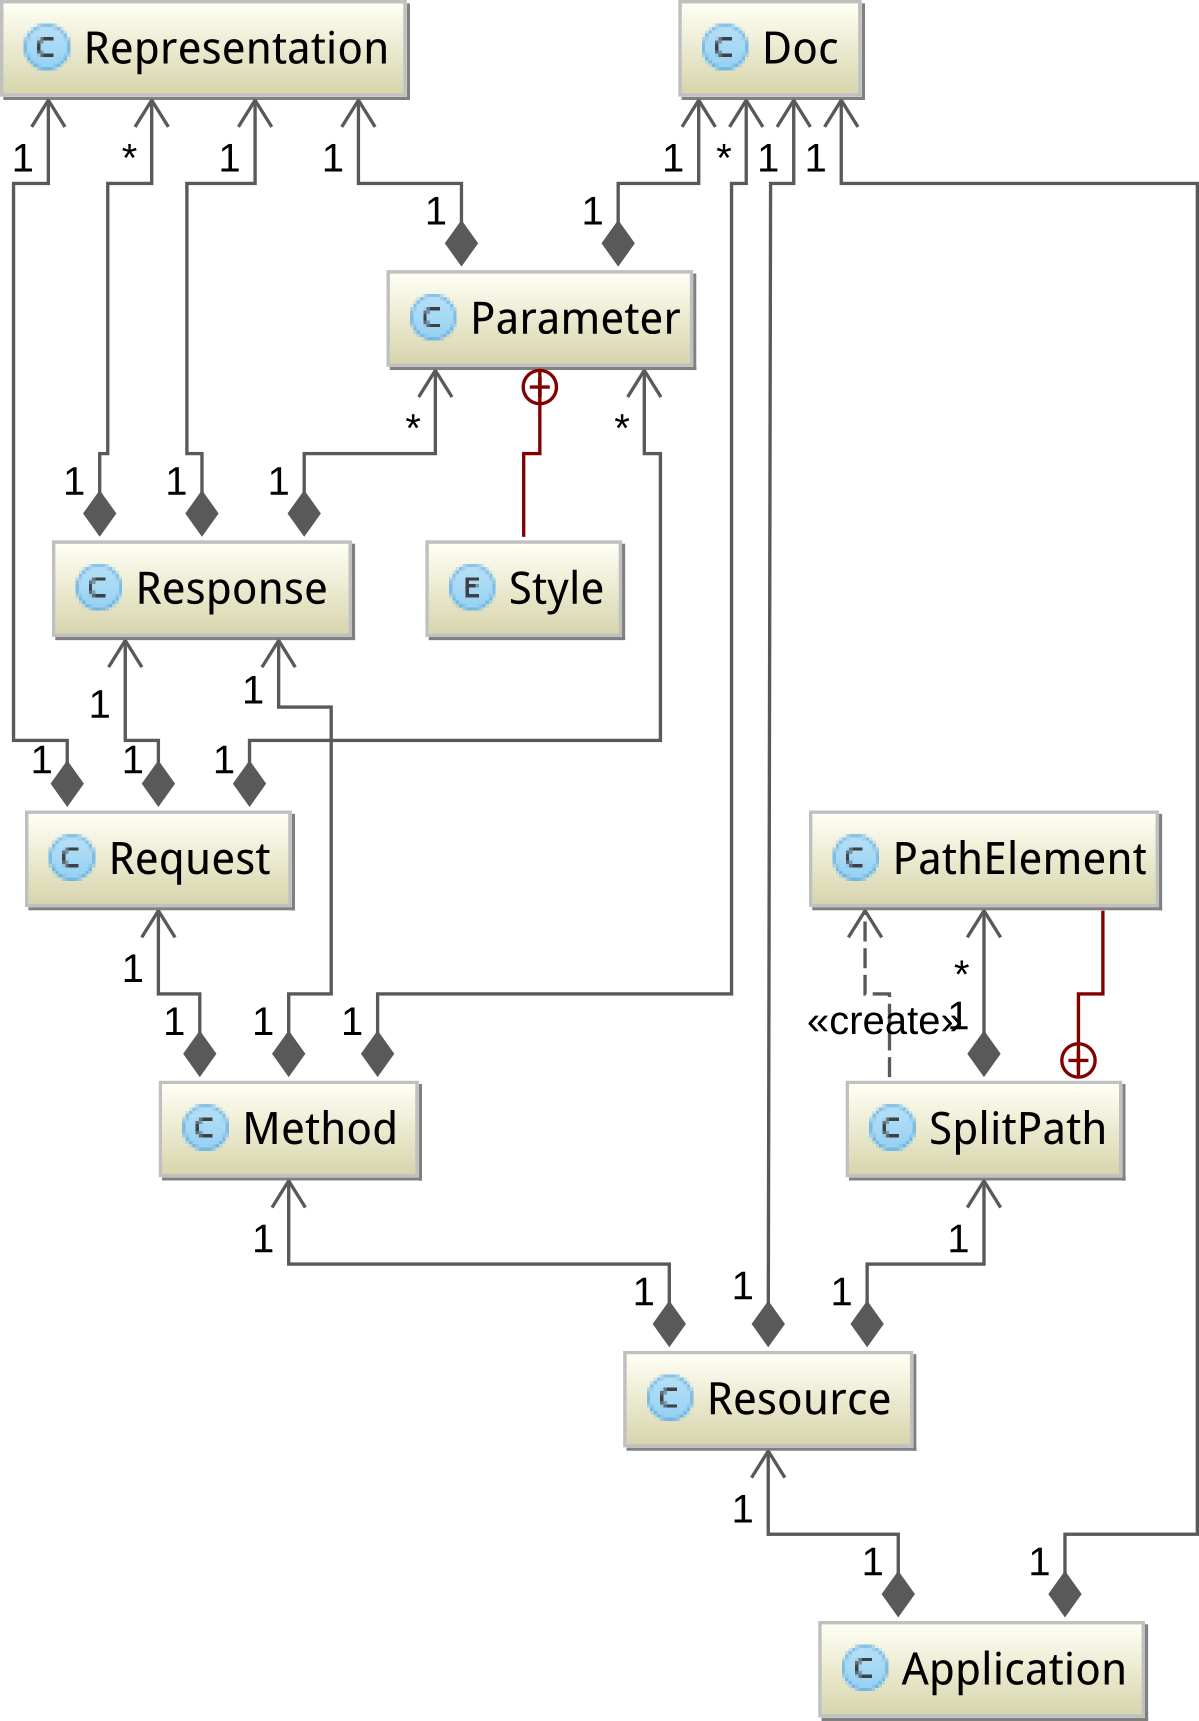
\includegraphics[width=0.5\textwidth]{resources/restmodel}
    \caption{UML Klassendiagramm des REST-Modells}
    \label{fig:restmodel}
\end{figure}

Wurzelelement des Modells (siehe \cref{fig:restmodel}) ist die Klasse \textbf{Application}, sie enthält \emph{Ressource}-Objekte und den Basisbezeichner der API bspw. \texttt{\small http://api.spreadshirt.net/api/v1/}. 

Eine \textbf{Ressource}-Klasse enthält eine Menge von \emph{Method}-Objekten, sowie einen Ressourcenbezeichner, dieser ist relativ zum Basisbezeichner des Wurzelelements. Die Ressourcenbezeichner können \emph{Template-Parameter} enthalten, diese werden bei einer Anfrage durch einen konkreten Wert ersetzt. Beispielweise enthält der Bezeichner für die Ressource eines bestimmten Users den Template-Parameter \{userid\}, vollständiger Ressourcenbezeichner \texttt{users/\{userid\}}. Ressourcenbezeichner werden durch die Klasse \textbf{SplitPath} repräsentiert. 

Jede \textbf{Method}-Klasse enthält ein \emph{Request} und ein \emph{Response} Objekt. Sie enthalten die nötigen Informationen für den Aufruf der Methode, bzw. über den Aufbau der Antwortnachricht.

Eine \textbf{Request}-Klasse enthält eine Liste von Query-Parametern sowie ein \emph{Representation} und \emph{Response} Objekt.

\textbf{Parameter} enthält Angaben zum \emph{Style}, Typ, Vorgabewert und ob dessen Angabe \enquote{required}, also notwendig ist. Die Angabe des Typs ist eine Referenz auf einen Typ aus einer XML-Schemabeschreibung. Der \emph{Style} gibt an wie der Parameter übermittelt wird, als Teil der Query \texttt{\ldots{}?mediaType=xml}, \emph{Key-Value Pair} des HTTP-Header oder als \emph{Template-Parameter} des Ressourcenbezeichners. 

Die Klasse \textbf{Response} enthält eine Liste mit \emph{Representation}-Objekten und Parameter-Objekten. Die Objekte vom Typ Representation enthalten die Beschreibung der Daten die bei einer erfolgreichen Anfrage an die Ressource zurückgesendet werden, sowie die der Fehlermeldung welche der Client anderenfalls erhält. Zwischen einer Fehlermeldung und einer erfolgreichen Anfrage kann anhand des Werts des HTTP-Statuscodes unterschieden werden. Erfolgreiche Anfragen liefern in der Antwort smeist einen Statuscode 200 \textbf{OK} oder 201 \textbf{Created} zurück, abhängig von der Anfragemethode. Die Response Parameter geben Einträge im HTTP-Header an, welche für den Client nützliche Informationen enthalten. Legt der Client z.B. via POST auf der Ressource \texttt{sessions} eine neue API-Session an, so enthält das Feld \texttt{Location} des HTTP-Headers der Serverantwort eine URL auf die Ressource der angelegten Session.

Die \textbf{Representation}-Klasse dient zur Beschreibung der Daten welche entweder zur API gesendet oder von dieser empfangen werden, sie besteht aus einer Angabe des \emph{media-type}, des HTTP-Statuscodes und eine Referenz auf die Definition des Datentyps. Das \emph{Representation}-Objekt des Request einer PUT- oder POST-Methode charakterisiert zum Beispiel den Aufbau der Daten welche der Ressource übermittelt werden, üblicherweise im HTTP-Body. Die Charakterisierung erfolgt dabei in Form einer Referenz auf einen Typ aus einer Schemabeschreibung sowie der Angabe des \emph{media-type}. Beispielsweise enthält das \emph{Representation}-Objekt der PUT-Methode auf Ressource \texttt{users/\{userId\}/designs/\{designId\}} den media-type \texttt{application/xml} und eine Referenz auf den Typ \texttt{sns:design}. 

Referenzen auf Typdeklaration aus einer Schemabeschreibung werden nachfolgend im Modell durch die konkrete Deklaration des Typs aus der XML-Schemabeschreibung ersetzt, siehe \cref{sec:application_model}. 

Ein Objekt der \textbf{Doc}-Klasse enthält einen Titel und eine Kurzbeschreibung des zugehörigen Elements.
Der Generator erzeugt daraus Quellcodekommentare für die Dokumentation der Bibliothek.

\subsection{Schema-Modell}
\label{sec:schema_model}

\begin{figure}[t]
    \centering
    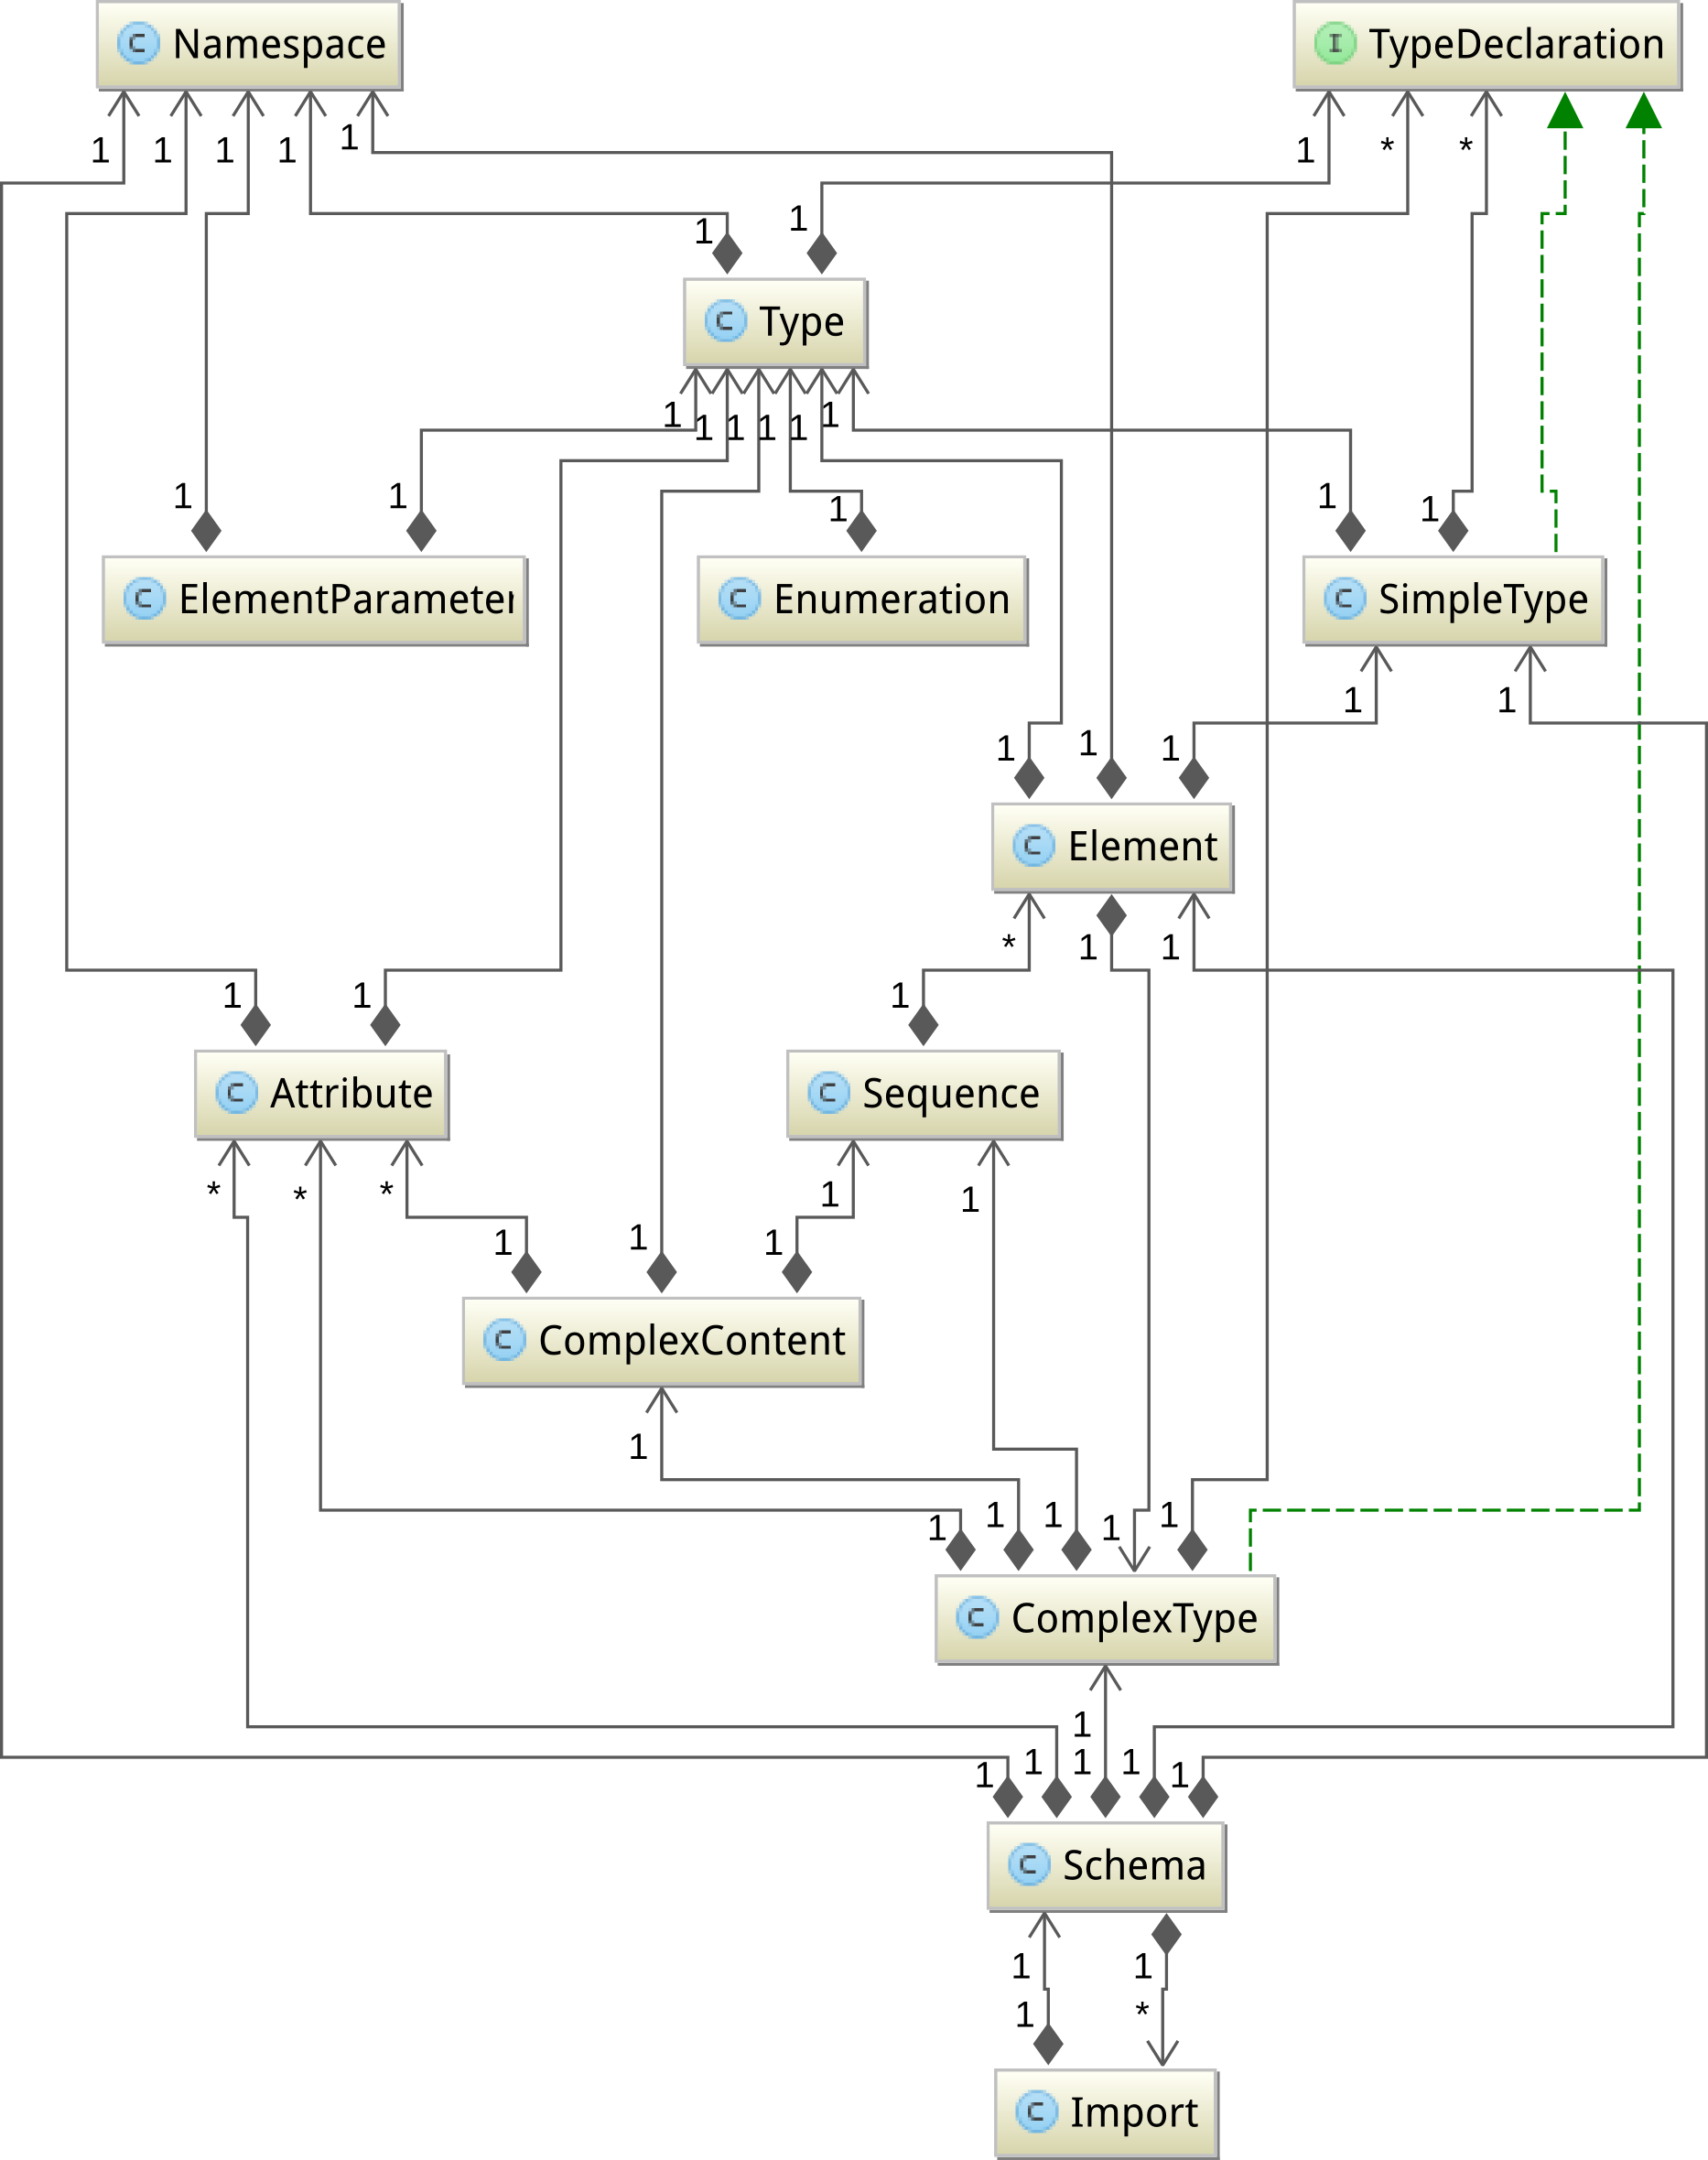
\includegraphics[width=0.6\textwidth]{resources/typemodel}
    \caption{\textsc{Uml} Klassendiagramm des Schemadatenmodells}
    \label{fig:schema_model}
\end{figure}

Wurzel des Schemadatenmodells ist die Klasse \textbf{Schema}. Ein Schema kann Objekte vom Typ \emph{Complex-} und \emph{SimpleType} sowie \emph{Attribute} und \emph{Element} enthalten.

\gls{XSD}-Dateien erlauben das Importieren anderer Schemadefinitionen, die Klasse \textbf{Import} ermöglicht dies im Schemamodell. Sie besitzt ein Objekt des zu importierenden Schemas sowie eine \gls{URI} auf die zugehörige \gls{XSD}-Datei.

Primitive Schematypen werden durch die Klasse \emph{SimpleType} abgebildet. Objekte dieser Klasse enthalten eine Kennzeichnung der Art des SimpleType (Enumerator, Liste, einfacher Wert) und bei Enumeratoren zusätzlich die einzelnen Enumeratorwerte sowie die Angabe des Basisdatentyps.

Die \textbf{ComplexType}-Klasse repräsentiert die gleichnamigen strukturierten Typen aus der Schemabeschreibung. 
Ein ComplexType kann Attribute, Elemente, Elementsequenzen und strukturierten Inhalt (\emph{ComplexContent}) enthalten.

\textbf{ComplexContent} kann die gleichen Objekte wie \emph{ComplexType} enthalten, sowie einen Basistyp der erweitert oder eingeschränkt wird (\enquote{derivation by extension/restriction}).

Attribute werden durch die gleichnamige Klasse \textbf{Attribute} gekapselt, sie besitzen einen Attributnamen sowie eine Definition ihres Typs.

Elementsequenzen werden durch die \textbf{Sequence}-Klasse repräsentiert. Sie enthält einen Reihenfolgeindikator und die Elemente der Sequenz.

Objekte der Klasse \textbf{Element} besitzen einen Bezeichner sowie einen Complex- oder SimpleType und optional eine Angabe der Auftrittshäufigkeit. Die Klasse \emph{ElementParameter} dient nur zur Kapselung der Daten, welche an den Konstruktor der Elementklasse gegeben werden.

Durch die Klasse \textbf{Namespace} werden der Namensraumbezeichner und der konkrete Namensraum eines Typs aus dem Schema gekapselt. 

\begin{figure}[ht]
    \centering
    \begin{minipage}[b]{0.6\linewidth}
        \begin{lstlisting}[
            language=XML,
            label=lst:xsdExamplePoint,                
            numbers=none,
            xleftmargin=0mm,
            framexleftmargin=2mm,
        ]
<xs:element 
    xmlns:tns="http://api.spreadshirt.net" 
    type="tns:point" name="point"/>

<xs:complexType name="point">
    <xs:sequence>
        <xs:element 
            type="xs:double" name="x"/>
        <xs:element 
            type="xs:double" name="y"/>
    </xs:sequence>
    <xs:attribute 
        xmlns:tns="http://api.spreadshirt.net" 
        type="tns:unit" name="unit"/>
</xs:complexType>
        \end{lstlisting}
    \end{minipage}
    \quad    
    \begin{minipage}[b]{0.35\linewidth}
        \begin{tikzpicture}[every tree node/.style={font=\footnotesize}]
            \Tree
            [
                .Element
                [
                    .ComplexType
                    [ . Attribute ]
                    [ .Sequence 
                        Element
                        [ .Element ]
                    ]
                ]
            ]
        \end{tikzpicture}
        %\label{fig:minipage2}
    \end{minipage}
    \caption{Datentyp Point mit Gegenüberstellung im Schemamodell}
\end{figure}

\subsection{Applikationsmodell}
\label{sec:application_model}

Das Applikationsmodell ist die Gesamtheit des \gls{REST}- und Schemamodells. Referenzen auf Typenbeschreibungen im \gls{REST}-Modell werden durch deren Definition im Schemamodell ersetzt. Dieses gemeinsame Modell dient dem Generator als Eingabequelle.

\subsection{Sprachenmodell}
\label{sec:language_model}

% Bild aktualisieren
\begin{sidewaysfigure}[tb]
    \centering
    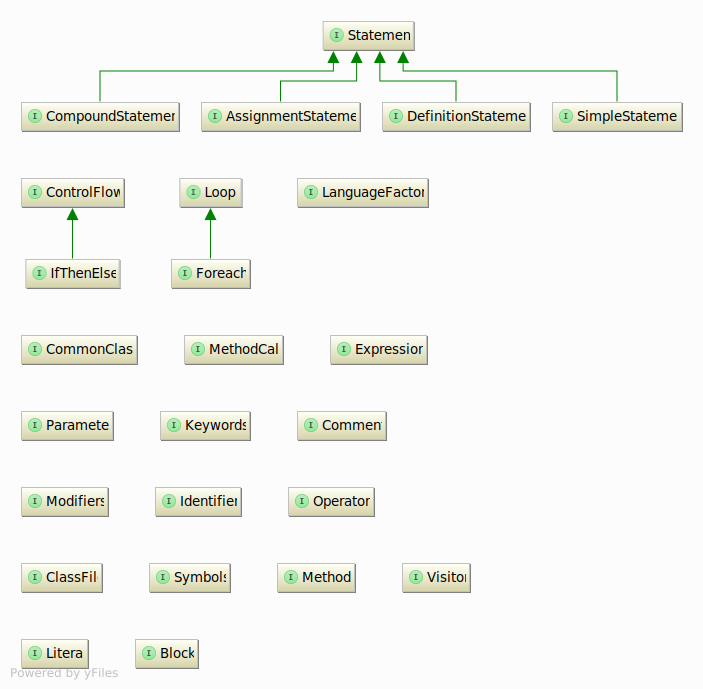
\includegraphics[width=\textwidth]{resources/languagemodel_common}
    \caption{UML Klassendiagramm des Zielsprachenmodells}
    \label{fig:language_model}
\end{sidewaysfigure}

Die Aufgabe des Generators ist die Transformierung des Applikationsmodells in das Modell der Zielsprache. 

Um die gewünschte Austauschbarkeit der Zielsprache zu gewährleisten wurde ein abstraktes Sprachenmodell entworfen welches die Konstrukte einer dateibasierten Objektorientierten Programmiersprache (siehe \cref{sec:oo_languages}) abbildet. 
%Anforderungen erstellen und referenzieren.
Die gewünschte Zielsprache muss dabei die Klassen und Methoden des Modells implementieren sowie eine \emph{Language Factory} (siehe \cref{sec:language_factory}) bereitstellen um vom Generator genutzt werden zu können.

Syntax ist kein Bestandteil des Modells sondern wird von einem \emph{LanguageVisitor} (siehe \cref{sec:language_visitor}) implementiert, das Sprachenmodell enthält nur die nötigen \emph{accept}-Methoden für den Visitor.

Basis des Modells ist die Klasse \textbf{ClassFile}, sie abstrahiert eine Klassendatei mit den Eigenschaften:
\begin{compactitem}
    \item Dateiname
    \item Namensraum
    \item Liste von Abhängigkeiten (\emph{Dependency}-Klasse)
    \item Klassendefinition
\end{compactitem}

Die Liste von Abhängigkeiten der zu generierenden Klassen muss vorher aus dem Eingabemodell ermittelt werden, dies geschieht durch Analyse der in den Elementdefinitionen des Schemamodells enthaltenen Typen. 

% Modifier sind Schlüsselwörter einer Sprache die deren Verhalten ändern.

\textbf{Keywords} und \textbf{Symbols} dienen zur Kapselung der Schlüsselwörter und Symbole einer Sprache. Keywords enthält Methoden zur Abfrage typischer Schlüsselworte wie \emph{class}, \emph{import}, \emph{new} oder \emph{this}. Sprachspezifische Symbole wie \emph{Verkettungs}- und \emph{Scope}-Operatoren oder Präfixe für Variablennamen können über Methoden der Klasse Symbols vom Generator abgefragt werden.

\subsection{Language Visitor}
\label{sec:language_visitor}

Kapitel gehört eher zu Generator

% Sprachschnittstelle!
\subsection{Language Factory}
\label{sec:language_factory}

Um eine Zielsprachenunabhänhigkeit zu erreichen, wird dem Generator bei der Erzeugung eine \enquote{Language Factory} übergeben. Der Generator erzeugt Sprachelemente nur über diese Factory. Ein Aufruf einer Factorymethode gibt ein Element der vom Typ der Sprache zurück, der Generator kennt aber nur den Interface-Typ. Für ihn ist die konkrete Implementierung somit transparent.


\section{Codegenerator}
\label{sec:codegenerator}

Nachdem in \cref{sec:concrete_models} die Datenmodelle des Generators betrachtet wurden, widmet sich dieser Abschnitt nur dem Aufbau des Codegenerators und den dort verwendeten Entwurfsmustern, \emph{Factory} (\cref{sec:language_factory}) und \emph{Visitor} (\cref{sec:language_visitor}). \Cref{fig:generation_process} zeigt ein Ablaufdiagramm des Generators.

\begin{sidewaysfigure}
    \centering
    \resizebox{ \textwidth}{!}{
        \begin{tikzpicture}[
        node distance=12mm and 8mm,
        every node/.style={font=\scriptsize}
    ]
    % Blocks
    \node(abstractDescription)[greyBlock]{Abstrakte\\Beschreibung\\der Spreadshirt-API};
    \node(dummy1)[dummy, right=of abstractDescription]{};
    \node(wadlAnalysis)[greyBlock, above right=of abstractDescription]{Analyse\\WADL-Datei};
    \node(restModel)[greyBlock, right=of wadlAnalysis]{REST-\\Modell};
    \node(xsdAnalysis)[greyBlock, below right=of abstractDescription]{Analyse\\XSD-Datei};
    \node(schemaModel)[greyBlock, right=of xsdAnalysis]{Schema-\\Modell};
    \node(modelCombine)[greyBlock, right=of dummy1]{Kombinierer};
    \node(applicationModel)[greyBlock, right=of modelCombine]{Applikations-\\Modell};
    \node(generator)[greyBlock, right=of applicationModel]{Generator};
    \node(languageModel)[greyBlock, right=of generator]{Zielsprachen-\\Modell};
    \node(languageFactory)[greyBlock, below=of generator]{Language Factory};
    \node(filePrinter)[greyBlock, right=of languageModel]{File Printer};
    \node(library)[greyBlock, double copy shadow, right=of filePrinter]{Bibliotheks-\\Dateien};

    %\node(languagemodel)[greyBlock, right= of generator]{Sprachenmodell\\\emph{Abstrakter Syntaxbaum}};
    % Lines  
    \path[arrow, ->] (abstractDescription) -- (wadlAnalysis);
    \path[arrow, ->] (abstractDescription) -- (xsdAnalysis);
    \path[arrow, ->] (wadlAnalysis) -- (restModel);
    \path[arrow, ->] (xsdAnalysis) -- (schemaModel);
    \path[arrow, ->] (restModel) -- (modelCombine);
    \path[arrow, ->] (schemaModel) -- (modelCombine);
    \path[arrow, ->] (modelCombine) -- (applicationModel);
    \path[arrow, ->] (applicationModel) -- (generator);
    \path[arrow, ->] (languageFactory) -- (generator);
    \path[arrow, ->] (generator) -- (languageModel);
    \path[arrow, ->] (languageModel) -- (filePrinter);
    \path[arrow, ->] (filePrinter) -- (library);

    %\path[arrow, ->] (infrastructurecode) -- (generator);
\end{tikzpicture}

    } 
    \caption{Ablaufdiagram des Generators}
    \label{fig:generation_process}
\end{sidewaysfigure}

\subsection{Language Factory}
\label{sec:language_factory}

Das \emph{Factory}-Pattern behandelt das Problem Familien von Objekten erzeugen zu wollen ohne die konkreten Klassen zu spezifizieren, sondern nur Interfaces festzulegen \cite[][S. 26]{patternsKompakt}.
Um eine Zielsprachenunabhängigkeit zu erreichen, wird dem Generator bei der Erzeugung eine Factory übergeben die das Interface \emph{Language Factory} des Sprachenmodells implementiert. 

Der Generator erzeugt Sprachelemente nur über diese Factory. Ein Aufruf einer Factorymethode gibt ein Sprachelement der Zielsprache zurück, der Generator kennt aber nur den Interface-Typ. Für ihn ist die konkrete Implementierung somit transparent. 
Die \emph{Language Factory} bildet damit die Schnittstelle zwischen dem Generator und der Implementierung des Zielsprachenmodells.

\subsubsection{Language Visitor}
\label{sec:language_visitor}

\citeauthor{patternsKompakt} definieren den Verwenduszweck des Patterns in \cite[][S. 60]{patternsKompakt} so: 
\thesisquote{Dieses Pattern ermöglicht es, neue Operationen auf den Elementen einer
Struktur zu definieren, ohne die Elemente selbst anzupassen.}

Die Aufgabe des \emph{Language Visitor} im Generator ist die Transformation des Sprachenmodells in eine Zeichenketten-Darstellung. Wie in \cref{sec:language_model} schon erwähnt, enthält die Klasse die das \emph{LanguageVisitor}-Interface implementiert, Regeln für eine syntaktisch korrekte Ausgabe des Sprachenmodells. Zusätzlich können in den LanguageVisitor \enquote{code conventions} implementiert werden, bspw. Einrückungstiefen, Zeilenlängen etc.

\subsection{Ausgabemodul}
\label{sec:printer_module}

Das Ausgabemodul beinhaltet Methoden zur Speicherung der Zeichenkettendarstellung aus dem \emph{Language Visitor}. Üblicherweise ist dies die Speicherung in Dateiform, es ist aber ebenso die Ausgabe auf \texttt{stdout} oder die Speicherung in einer Datenbank möglich.

%\section{API-Design}
\label{sec:api-design}

\subsection{Kriterien}
\label{sec:design_criterias}

\subsection{Sessions}
\label{sec:sessions}

\subsection{Parameterobjekte}
\label{sec:parameter_objects}

\subsection{Entwurfsmuster}
\label{sec:patterns}

\subsubsection{Expression Builder}
\label{sec:expression_builder}

\subsubsection{Fluent Interface}
\label{sec:fluent_interface}


    \chapter{Evaluation}
\label{chap:evaluation}

\chapterQuote{There are two ways to write error-free programs; only the third one works}{\citeauthor{alanPerlis}}{\citeyear{alanPerlis}}{\cite{alanPerlis}}

Die Bewertung --- oder auch Evaluierung --- der generierten Client-Bibliothek gegenüber den Anforderungen (siehe \cref{item:requirements}) anhand von Anwendungsbeispielen ist Bestandteil dieses Kapitels.

% todo: Überschrift ändern
\section{PHP-Zielsprachenmodell}
\label{sec:php_target_language_model}

\Cref{fig:modelRepresentationOfBatchDTO} zeigt die Gegenüberstellung von \Cref{lst:batchDTO} in Form des \gls{AST} der durch das Sprachmodell gebildet wird. 

\begin{lstlisting}[
    language=PHP,
    caption=Ausschnitt der Datenklasse BatchDTO,
    label=lst:batchDTO
]
<?php
   require_once('Dto.php');
   require_once('OperationDTO.php');

   class BatchDTO
   {
      private $operations = array(); // operationDTO 
      ...
      public static function fromXML(
            /* SimpleXMLElement */ $xml
         )
      {
         $operations = OperationDTO::fromXML(/* SimpleXMLElement */ $xml->operations);
          ...
      }
      ...
   }
?>
\end{lstlisting}

\begin{sidewaysfigure}
    \centering
    \resizebox{1.0\textheight}{!}{
      \begin{tikzpicture}[every tree node/.style={font=\ttfamily}]    
    \Tree
    [.ClassFile 
        [ .Import 
            [ .Literal 
                [ .PrimitiveType 
                    {'Dto.php'}
                ] 
            ]            
        ]
        [ .Import 
            {\ldots}
        ]    
        [ .CommonClass
            {'BatchDTO'}
            [
                .AssignmentStatement
                [ .Variable
                    {"operations"}
                    [ .Modifiers
                        {"private"}
                    ]
                ]
                [ .Operator 
                    {"="}
                ]                
                [
                    .MethodInvocation
                    {"array"}
                ]
            ]
            [
                .DefinitionStatement        
                {"fromXML"}
                [
                    .Modifiers
                    {"public"}
                    {"static"}
                ] 
                [ .Identifier
                    [ .Comment
                        {"SimpleXMLElement"}
                    ]
                    {"xml"}
                ]
                [
                    .Block
                    [
                        [ .AssignmentStatement 
                            [ .Identifier
                                {"operations"}
                            ]
                            [ .Operator
                                {"="}
                            ]
                            [ .SimpleExpression
                                [ .Identifier
                                    {"OperationDTO"}
                                ]                
                                [ .Operator 
                                    {"::"}
                                ]
                                [
                                    .MethodInvocation
                                    {"fromXML"}
                                    [                                                
                                        .SimpleExpression                                                
                                        [ .Identifier
                                            [ .Comment
                                                {"SimpleXMLElement"}
                                            ]
                                            {"xml"}
                                        ]
                                        [ .Operator
                                            {"->"}
                                        ]
                                        [ .Identifier   {"operations"}
                                        ]
                                    ]
                                ]
                            ]
                        ]                                                    
                    ]
                ]
            ]            
        ]
    ]
\end{tikzpicture}
    }
    \caption{Darstellung von BatchDTO aus \Cref{lst:batchDTO} im Sprachenmodell}
    \label{fig:modelRepresentationOfBatchDTO}
\end{sidewaysfigure}

\section{Nutzbarkeit}
\label{sec:usability}

Derzeit ist die Bibliothek noch eingeschränkt nutzbar, da die De-/Serialisier von strukturierten Typen noch nicht fehlerfrei generiert werden. Die Informationen die nötig sind um Datenklassen verlustfrei zu serialisieren bzw. deren \textsc{Xml}-Repräsentation zu deserialisieren sind im Schema-Modell (siehe \cref{sec:schema_model}) vorhanden, der Algorithmus im Codegenerator zur Erzeugung dieser Methoden muss deshalb überarbeitet werden.

\section{Leistungsbewertung}
\label{sec:performance_measurement}

\begin{lstlisting}[
    language=PHP,
    caption=Beispiel für eine Interaktion mit der Spreadshirt-API über die generierte Client-Bibliothek,
    label=lst:giveMeALabel
]
<?php

require_once("data/LoginDTO.php");
require_once("resources/UsersUserId.php");
require_once("resources/Sessions.php");

$userId = "1234567";
$apiKey = "098fc12a-0777-426f-b47c-a7bb872cdf09";
$secret = "ba125903-68b2-4f3b-93ae-a83090e20ce8";

$loginDTO = new LoginDTO();
$loginDTO->setUsername("username");
$loginDTO->setPassword("password");
$resource = new Sessions();
$session = $resource->POST(null, $loginDTO);

$user = new UsersUserId($userId);

?>
\end{lstlisting}

%\section{Codemetriken}
%\label{sec:codemetrics}
    \chapter{Implementierung}

\section{XML-Parser}

DOM-Parser vs. Streaming-Parser
    \chapter{Schlussbetrachtung}
\label{chap:summary}

\chapterQuote{The most important property of a program is whether it accomplishes the intention of its user.}{\citeauthor{hoareAxiomatic}}{\citeyear{hoareAxiomatic}}{\cite[][S. 4]{hoareAxiomatic}}

Das Ziel dieser Arbeit war die Erstellung eines Codegenerators mit flexibler Zielsprache der aus einer abstrakten Beschreibung eines \gls{RESTful} Web Service eine Client-Bibliothek erzeugen sollte. Dies geschah am Beispiel der Spreadshirt-\gls{API} mit \textsc{Php} als Zielsprache der Bibliothek. 
Während der Bearbeitung der Aufgabenstellung stellten sich die folgenden vier Schwerpunkte heraus:
\begin{compactitem}
    \item Erstellung von Datenmodellen für die abstrakte Web Service Beschreibung
    \item Überführung der abstrakten Web Service Beschreibung in die Datenmodelle
    \item Analysieren der Konzepte von objektorientierten Programmiersprachen zur Erzeugung eines Sprachenmodells
    \item Design der Client-Bibliothek auf einfache Nutzung optimieren (beispielweise durch Integration der \gls{API}-Autorisierung)
\end{compactitem}

Der im Rahmen dieser \thesisDesignator{} aus den gewonnen Erkenntnissen entwickelte Codegenerator erzeugt aus der abstrakten Beschreibung der Spreadshirt-\gls{API} eine Client-Bibliothek, die derzeit, wenn auch in eingeschränktem Umfang, nutzbar ist. Da der Generator zielsprachenunabhängig arbeitet, kann er durch Implementierung eines Sprachenmodells eine Client-Bibliothek in einer neuen objektorientierten Zielsprache erzeugen. Durch die Trennung von Syntax und Semantik im Sprachenmodell, ließen sich mit geringem Aufwand Konventionen für den \enquote{code style} der generierten Bibliothek festlgegen. Dies resultiert in gut lesbaren Quellcode der erzeugten Klassen.

Die Aufgabenstellung war umfangreich und fordernd, aber dennoch lösbar. Die Erstellung des Sprachenmodells bedurfte der Auseinandersetzung mit grundlegenden Programmiersprachkonzepten und den Grundlagen des Compilerbaus.

%Im Verlauf dieser \thesisDesignator{} konnten die allgemeinen Konzepte von Web Services, Dokumentbeschreibungssprachen und Codegeneratoren erläutert werden. Aus den beschriebenen Grundlagen konnten Datenmodelle erstellt werden, welche als Ein- und Ausgabemodell des Generators dienen. Das Eingabedatenmodell enthielt die Spreadshirt-\gls{API} Beschreibung und das Ausgabemodell abstrahierte die zu generierende Zielsprache. Im weiteren wurde auch der Ablauf der Codegenerierung besprochen und in einem Diagramm veranschaulicht (\cref{fig:generation_process}). Eine Evaluierung der erzeugten Bibliothek gegenüber den Anforderungen fand ebenfalls statt.

%Im Verlauf dieser \thesisDesignator{} konnte das Zusammenwirken von Datenmodellen und einem 
%Im Verlauf dieser \thesisDesignator{} konnte gezeigt werden wie mit Hilfe der Grundlagen über Web Services, Dokumentbeschreibungs- und objektorientierte Programmiersprachen, darauf basierende Datenmodelle erstellt wurden. 
%Anhand dieser \thesisDesignator{} konnte die Vorgehensweise gezeigt werden ...
%Erstellung einer Client-Bibliothek aus der abstrakten Beschreibung eines Web Services.
%Der entwickelte Codegenerator zur Erzeugung einer Client-Bibliothek für die Spreadshirt-\gls{API} \ldots\\
%Vorteile die sich daraus ergeben\ldots\\

%Schwierigkeiten und Probleme bei der Erstellung\ldots
%    In neue Programmiersprache einarbeiten
%    Überführen der Beschreibung in ein geeignetes Modell
%    Komplexität des Sprachenmodells (Konzepte der Programmiersprachen, Gemeinsamkeiten herausarbeiten)
%    Erstellung des Generators aufwendig 

\section{Ausblick}
\label{sec:prospect}

% todo: implementierung anderer Sprachmodelle, Schnittstelle zu Generator

Der in dieser Arbeit dokumentierte Codegenerator bietet mehrere Ansatzpunkte für Erweiterungen oder Verbesserungen:

\begin{compactitem}
    \item Generierung eines \emph{Fluent-Interface} Pattern. Dieses Entwurfsmuster wurde von \citeauthor{fowler2010domain} in \cite{fowler2010domain} beschrieben und basiert auf der Technik des \enquote{method-chaining}, also der Hintereinanderausführung von Methoden, wobei jede Methode mit dem Resultat der vorangegangen arbeitet.
    \item Die Erzeugung von Parameterobjekten welche die Parametersignatur der jeweiligen Methode repräsentieren, wird verhindert das der Nutzer unerlaubte Parameter an eine Methode übergibt. Dies ist derzeit möglich, da vom Nutzer beliebiger Inhalt die Arrays eingetragen werden kann, die zur Übermittlung der Methodenparameter dienen.
    \item Implementieren weiterer Sprachenmodelle, bspw. zur Generierung einer Java-Bibliothek. 
    \item Erzeugen von Tests durch den Generator um die generierte Bibliothek automatisch prüfen zu können.
\end{compactitem}
\label{sec:prospect}

%\section{Fazit}

%\label{sec:conclusion}

    \label{lastPage}
}
\blankpage


% Beginn des Anhangs
\renewcommand*{\chapterpagestyle}{appendixChapterStyle}
{   
    % remove cleardoublepage for appendix     
    \let\cleardoublepage\relax
    \appendix 
    \pagestyle{appendixStyle}
    \pagenumbering{Alph}

    % Glossar        
    \glsaddall
    \printglossary[type=main,title={Glossar},toctitle={Glossar}]
    \newpage
    % Bilderverzeichnis
        %\cleardoublepage
    \addcontentsline{toc}{chapter}{\listfigurename}
    \listoffigures
    \newpage
    % Tabellenverzeichnis
        %\cleardoublepage
    \addcontentsline{toc}{chapter}{\listtablename}
    \listoftables
    \newpage    
    % Listingverzeichnis
    \addcontentsline{toc}{chapter}{\lstlistlistingname}
    \lstlistoflistings
    \newpage    
    % Definitionsverzeichnis
    \addcontentsline{toc}{chapter}{\listtheoremname}
    \listoftheorems
    \newpage    
    % Literaturverzeichnis
        %\cleardoublepage
    \addcontentsline{toc}{chapter}{\bibname}
    %
% books.google.com
%

%books without citations wont be printed otherwise
\nocite{*}
\printbibliography

    \newpage
    \chapter*{\BibTeX{} Eintrag}
\addcontentsline{toc}{chapter}{\BibTeX{} Eintrag}

%ToDo: upload thesis or change the url :)
\begin{lstlisting}[
	language=TeX,
	backgroundcolor=\color{white},
	keywordstyle=\color{black},
	identifierstyle=\color{black},
	numbers=none,
	frame=none
]
@phdthesis{AndreasLinz2013,
	type = {//@\thesisDesignator@//}
	author = {Linz, Andreas},
	year = {//@\the\year@//},
	month = {//@\the\month@//},
	day = {//@\the\day@//},
	timestamp = {//@\the\year\the\month\the\day@//},
	title = {//@\thesisTitle{}@//},
	school = {HTWK-Leipzig},
	pdf = {http://www.klingt.net/bachelor/thesis/thesis.pdf}
}
\end{lstlisting}
    
    \label{lastAppendixPage}
}

%
% Ende der Thesis 
%